\chapter{Project host on GitHub / GitLab}
\label{hosting}

The previous chapter introduced Git a powerful tool for managing code changes. \\
Its real interest comes to light if you want your project to be collaborative,  
and/or if you want to publish your source code. \\
Indeed in that case you need to think about hosting your project, that is your Git repository on-line, 
or at least in a remote location where every contributor, member of your community, can access the source code. \\
The 2 most famous dedicated websites for that purpose are \github\ and \gitlab.

\section{Introduction and user setup}

The first step is to create a user account on the platform of you choice. \\
I will skip details on the registration process, however when the account is created you will see something that looks like:
\begin{itemize}
\item \github: \\[0.25cm]

\includegraphics[width=0.85\textwidth,keepaspectratio=true,draft=\ddst]{img/hosts/github/home.eps}
\item \gitlab: \\[0.25cm]
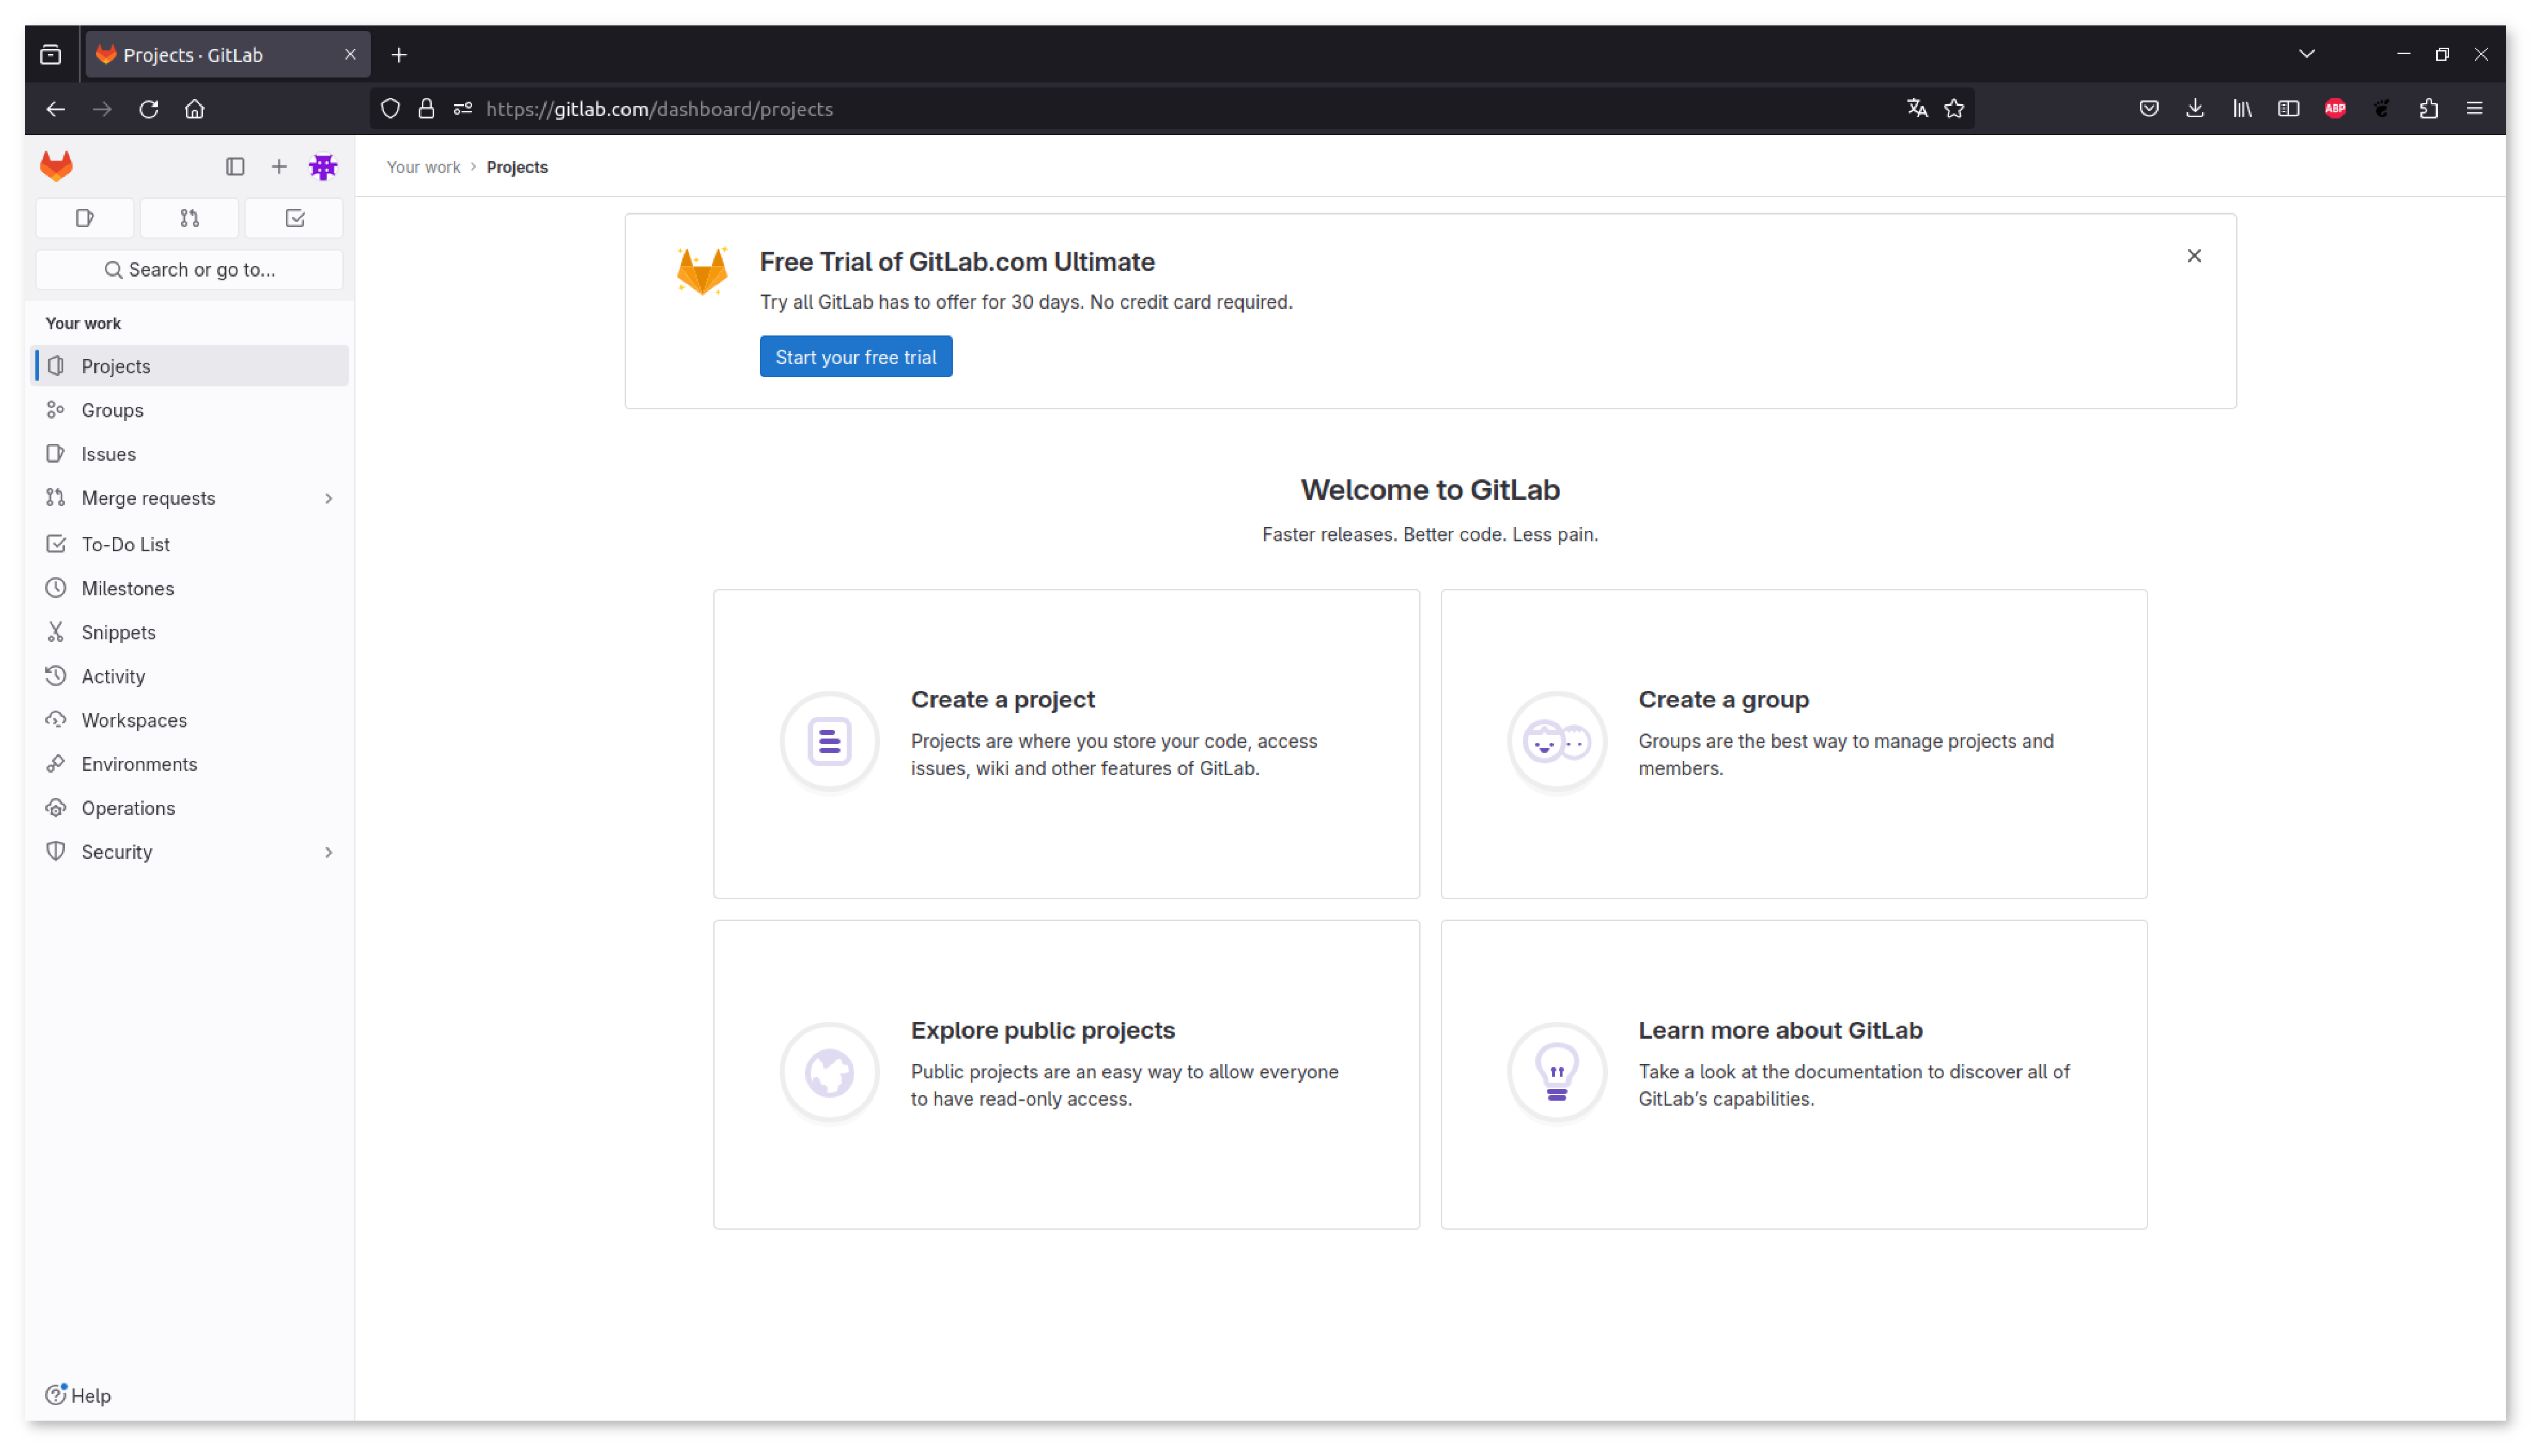
\includegraphics[width=0.85\textwidth,keepaspectratio=true,draft=\ddst]{img/hosts/gitlab/home.eps}
\end{itemize}
In the following examples for both \github\ and \gitlab:
\begin{itemize}
\item the account/group name is: "\texttt{TTPSLR}"
\item the project name is: "\texttt{Program}"
\end{itemize}

\newpage
\section{Creating a repository / project}

The procedure is quite similar, only the denomination changes: 
\begin{itemize}
\item On \github\ the space to store and share your sources is called a "\texttt{repository}"
\item On \gitlab\ the space to store and share your sources is called a "\texttt{project}"
\end{itemize}
\vspace{0.25cm}
\begin{itemize}
\item \github:
\end{itemize}
\vspace{0.5cm}
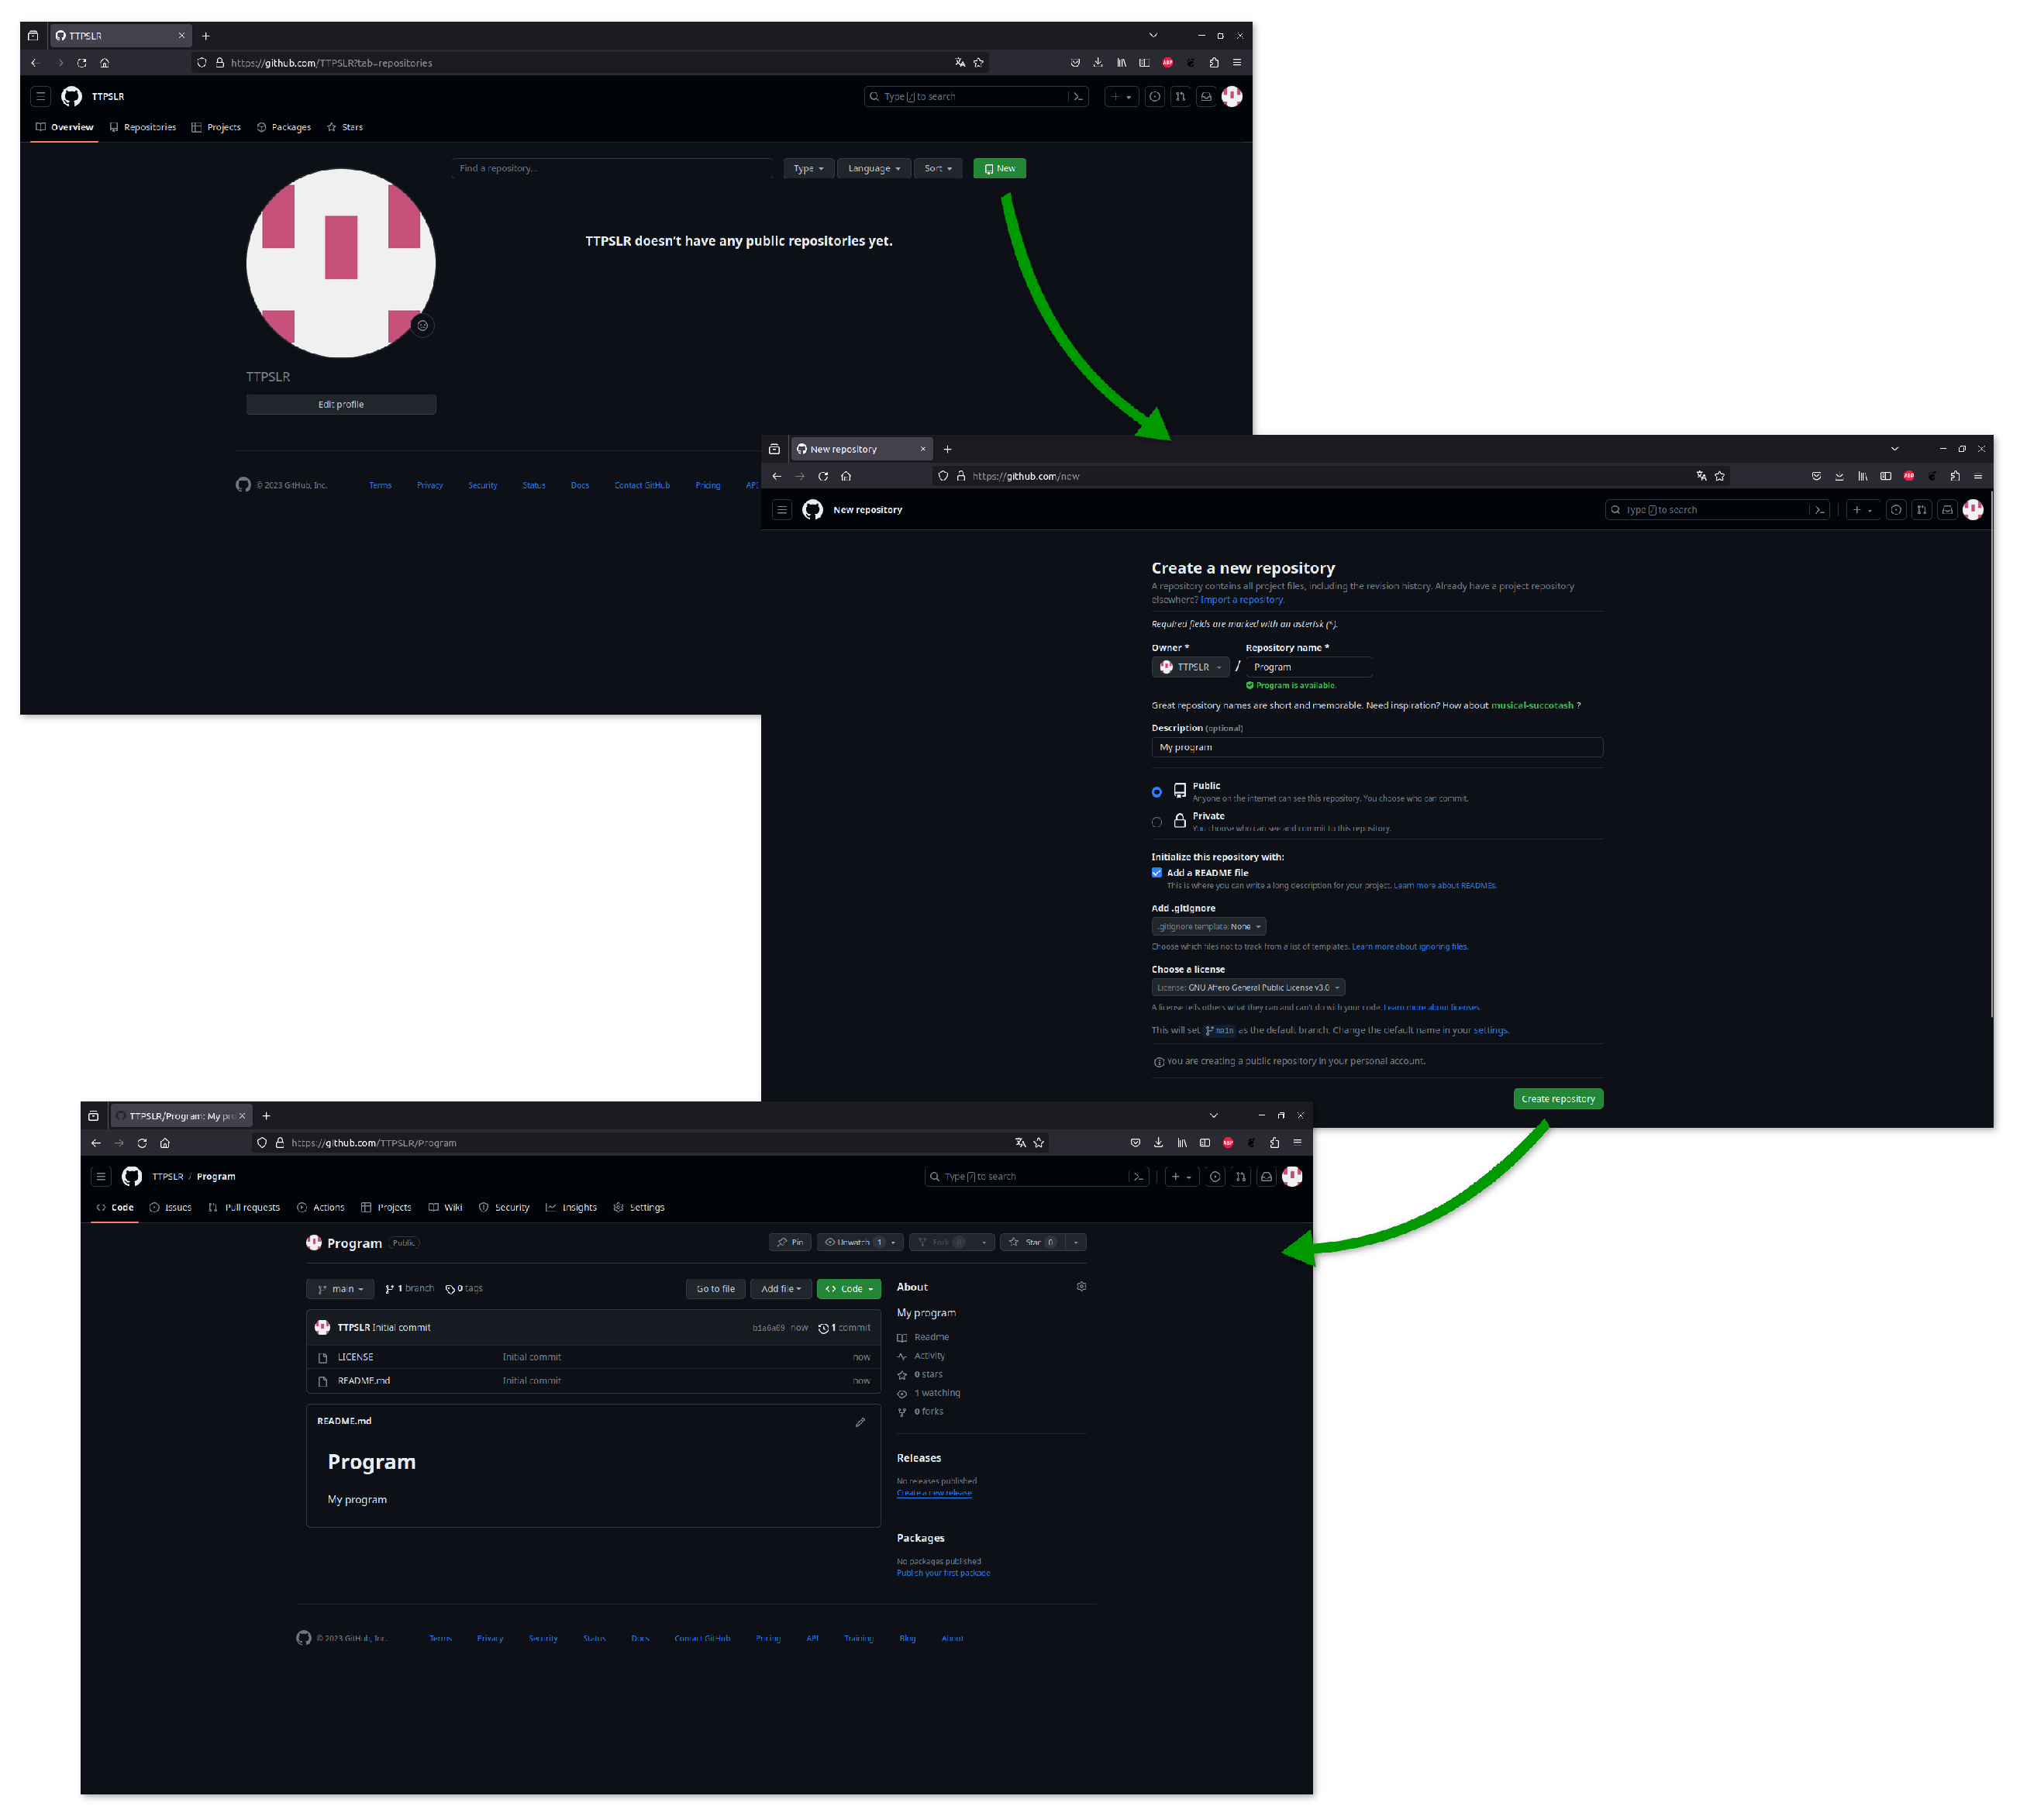
\includegraphics[width=1.0\textwidth,keepaspectratio=true,draft=\ddst]{img/hosts/github/new-p.eps} \\[0.25cm]
\begin{itemize}
\item Open the "\texttt{Repositories}" tab and click on "\texttt{New}"
\item Fill the new project information
\item Click on "\texttt{Create repository}"
\end{itemize}
\newpage
\begin{itemize}
\item \gitlab:
\end{itemize}
\vspace{0.5cm}
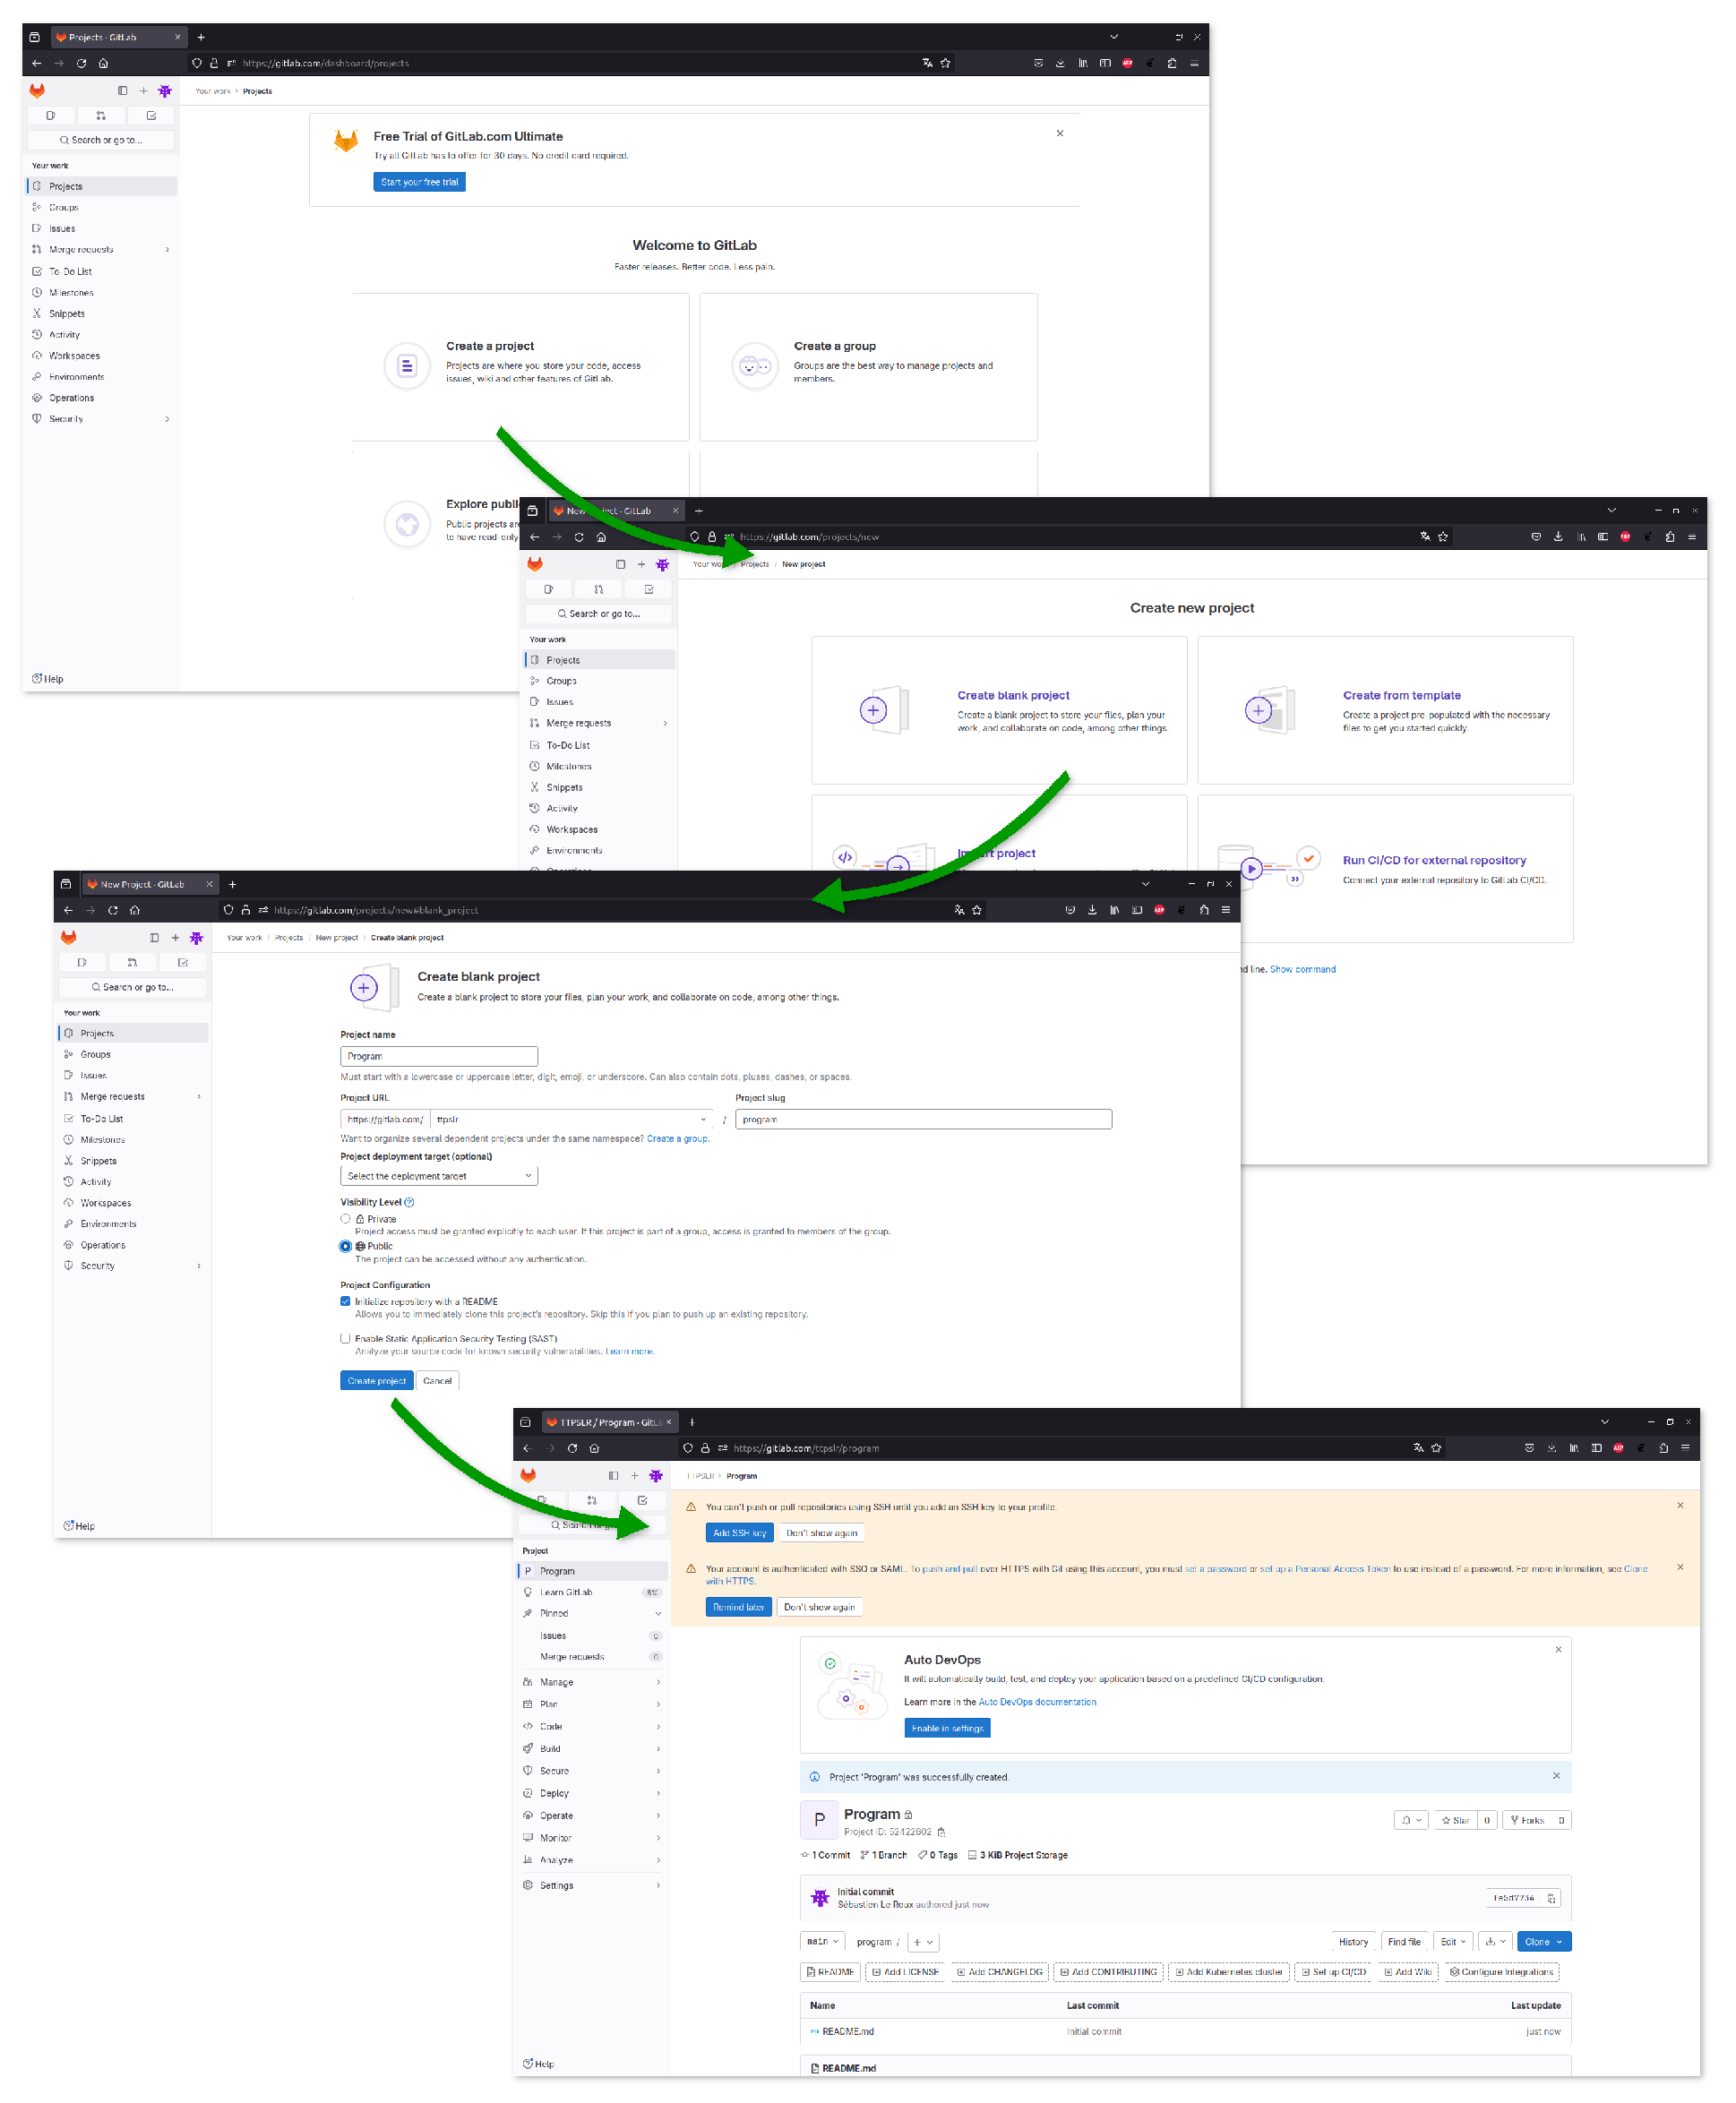
\includegraphics[width=1.0\textwidth,keepaspectratio=true,draft=\ddst]{img/hosts/gitlab/new-p.eps} %\\[0.25cm]
\newpage
\begin{itemize}
\item Click on "\texttt{Create project}"
\item Click on "\texttt{Create blank project}"
\item Fill the new project information
\item Click on "\texttt{Create project}"
\end{itemize}

\section{SSH encryption keys}

Immediately after creating your first project, setup the SSH encryption keys. 
These keys are digital tokens that prove your identity when performing actions to update the on line repository using Git. 

\subsection{Generating SSH encryption keys}

If not done already you need first to create SSH encryption keys, this is done using a command line utility: 
\begin{script}
\fprompt{~} \bftt{ssh-keygen} \rtt{-t} \dgtt{ed25519}
\end{script}
"\bftt{ssh-keygen}" generates the key, the "\rtt{-t}" option is used to define the type of encoding, in the example "\dgtt{ed25519}" that stands for \href{https://en.wikipedia.org/wiki/EdDSA}{Edwards-curve Digital Signature Algorithm} which is the most secured standardization these days.  \\
2 files, to be stored in "\texttt{\textasciitilde/.ssh}", will be created by the previous command:
\begin{itemize}
\item A private key, that decipher (act like a key), and that must remains on your computer: 
\begin{scripti}
~/.ssh/id\_ed25519
\end{scripti} \\
\vspace{-1.5cm}
\item A matching public key, that encrypts (acts like a door), used on remote system(s):
\begin{scripti}
~/.ssh/id\_ed25519.pub
\end{scripti} \\[-0.65cm]
\noindent Which content looks like: 
{\scriptsize{
\begin{scripti}
\fprompt{~} cat ~/.ssh/id\_ed25519.pub
ssh-ed25519 AAAAC3NzaC1lZDI1NTE5AAAAIG1TIYyaRZIlFU40NH8QAxXK8SSgl07Thop6CGzcVg0j user@host
\end{scripti}}} \\
\vspace{-1.5cm}
\end{itemize}
For more about asymmetric keys algorithms: \href{https://en.wikipedia.org/wiki/Public-key\_cryptography}{https://en.wikipedia.org/wiki/Public-key\_cryptography}
\newpage

\subsection{Adding the keys to GitHub / GitLab}

Now you need to add the public key to your \github\ / \gitlab\ repository: 
\begin{itemize}
\item \github\ (see figure~\ref{kgithub}):
\begin{itemize}
\item Click on the profile logo and click on "\texttt{Settings}"
\item Click on the "\texttt{SSH and GPG keys}"
\item Click on "\texttt{Create repository}"
\item Click on "\texttt{New SSH key}"
\item Adjust the key information:
\begin{itemize}
\item Give the key a title name
\item Select the key type: "\texttt{Authentication key}" 
\item Copy / paste the content of public key file in the text box
\end{itemize}
\item Finally click on "\texttt{Add SSH key}"
\end{itemize}
\item \gitlab\ (see figure~\ref{kgitlab}):
\begin{itemize}
\item Click on shortcut button "\texttt{Add SSH key}" \\
Alternatively click on your public avatar (squared in red in figure~\ref{kgitlab}), \\
click on "\texttt{Preferences}", then click on "\texttt{SSH Keys}"
\item Click on the "\texttt{Add new key}"
\item Adjust the key information:
\begin{itemize}
\item Copy / paste the content of public key file in the text box
\item Give the key a title name
\item Select the key type: "\texttt{Authentication}" or "\texttt{Authentication \& Signing}" 
\end{itemize}
\item Finally click on "\texttt{Add key}"
\item Optionally go back the "\texttt{User Settings} $\Longrightarrow$ \texttt{SSH Keys}" tab to visualize that the key is properly stored
\end{itemize}
\end{itemize}
As soon as the keys have been installed you are ready to work with your on line repository. 

\begin{figure}[!p]
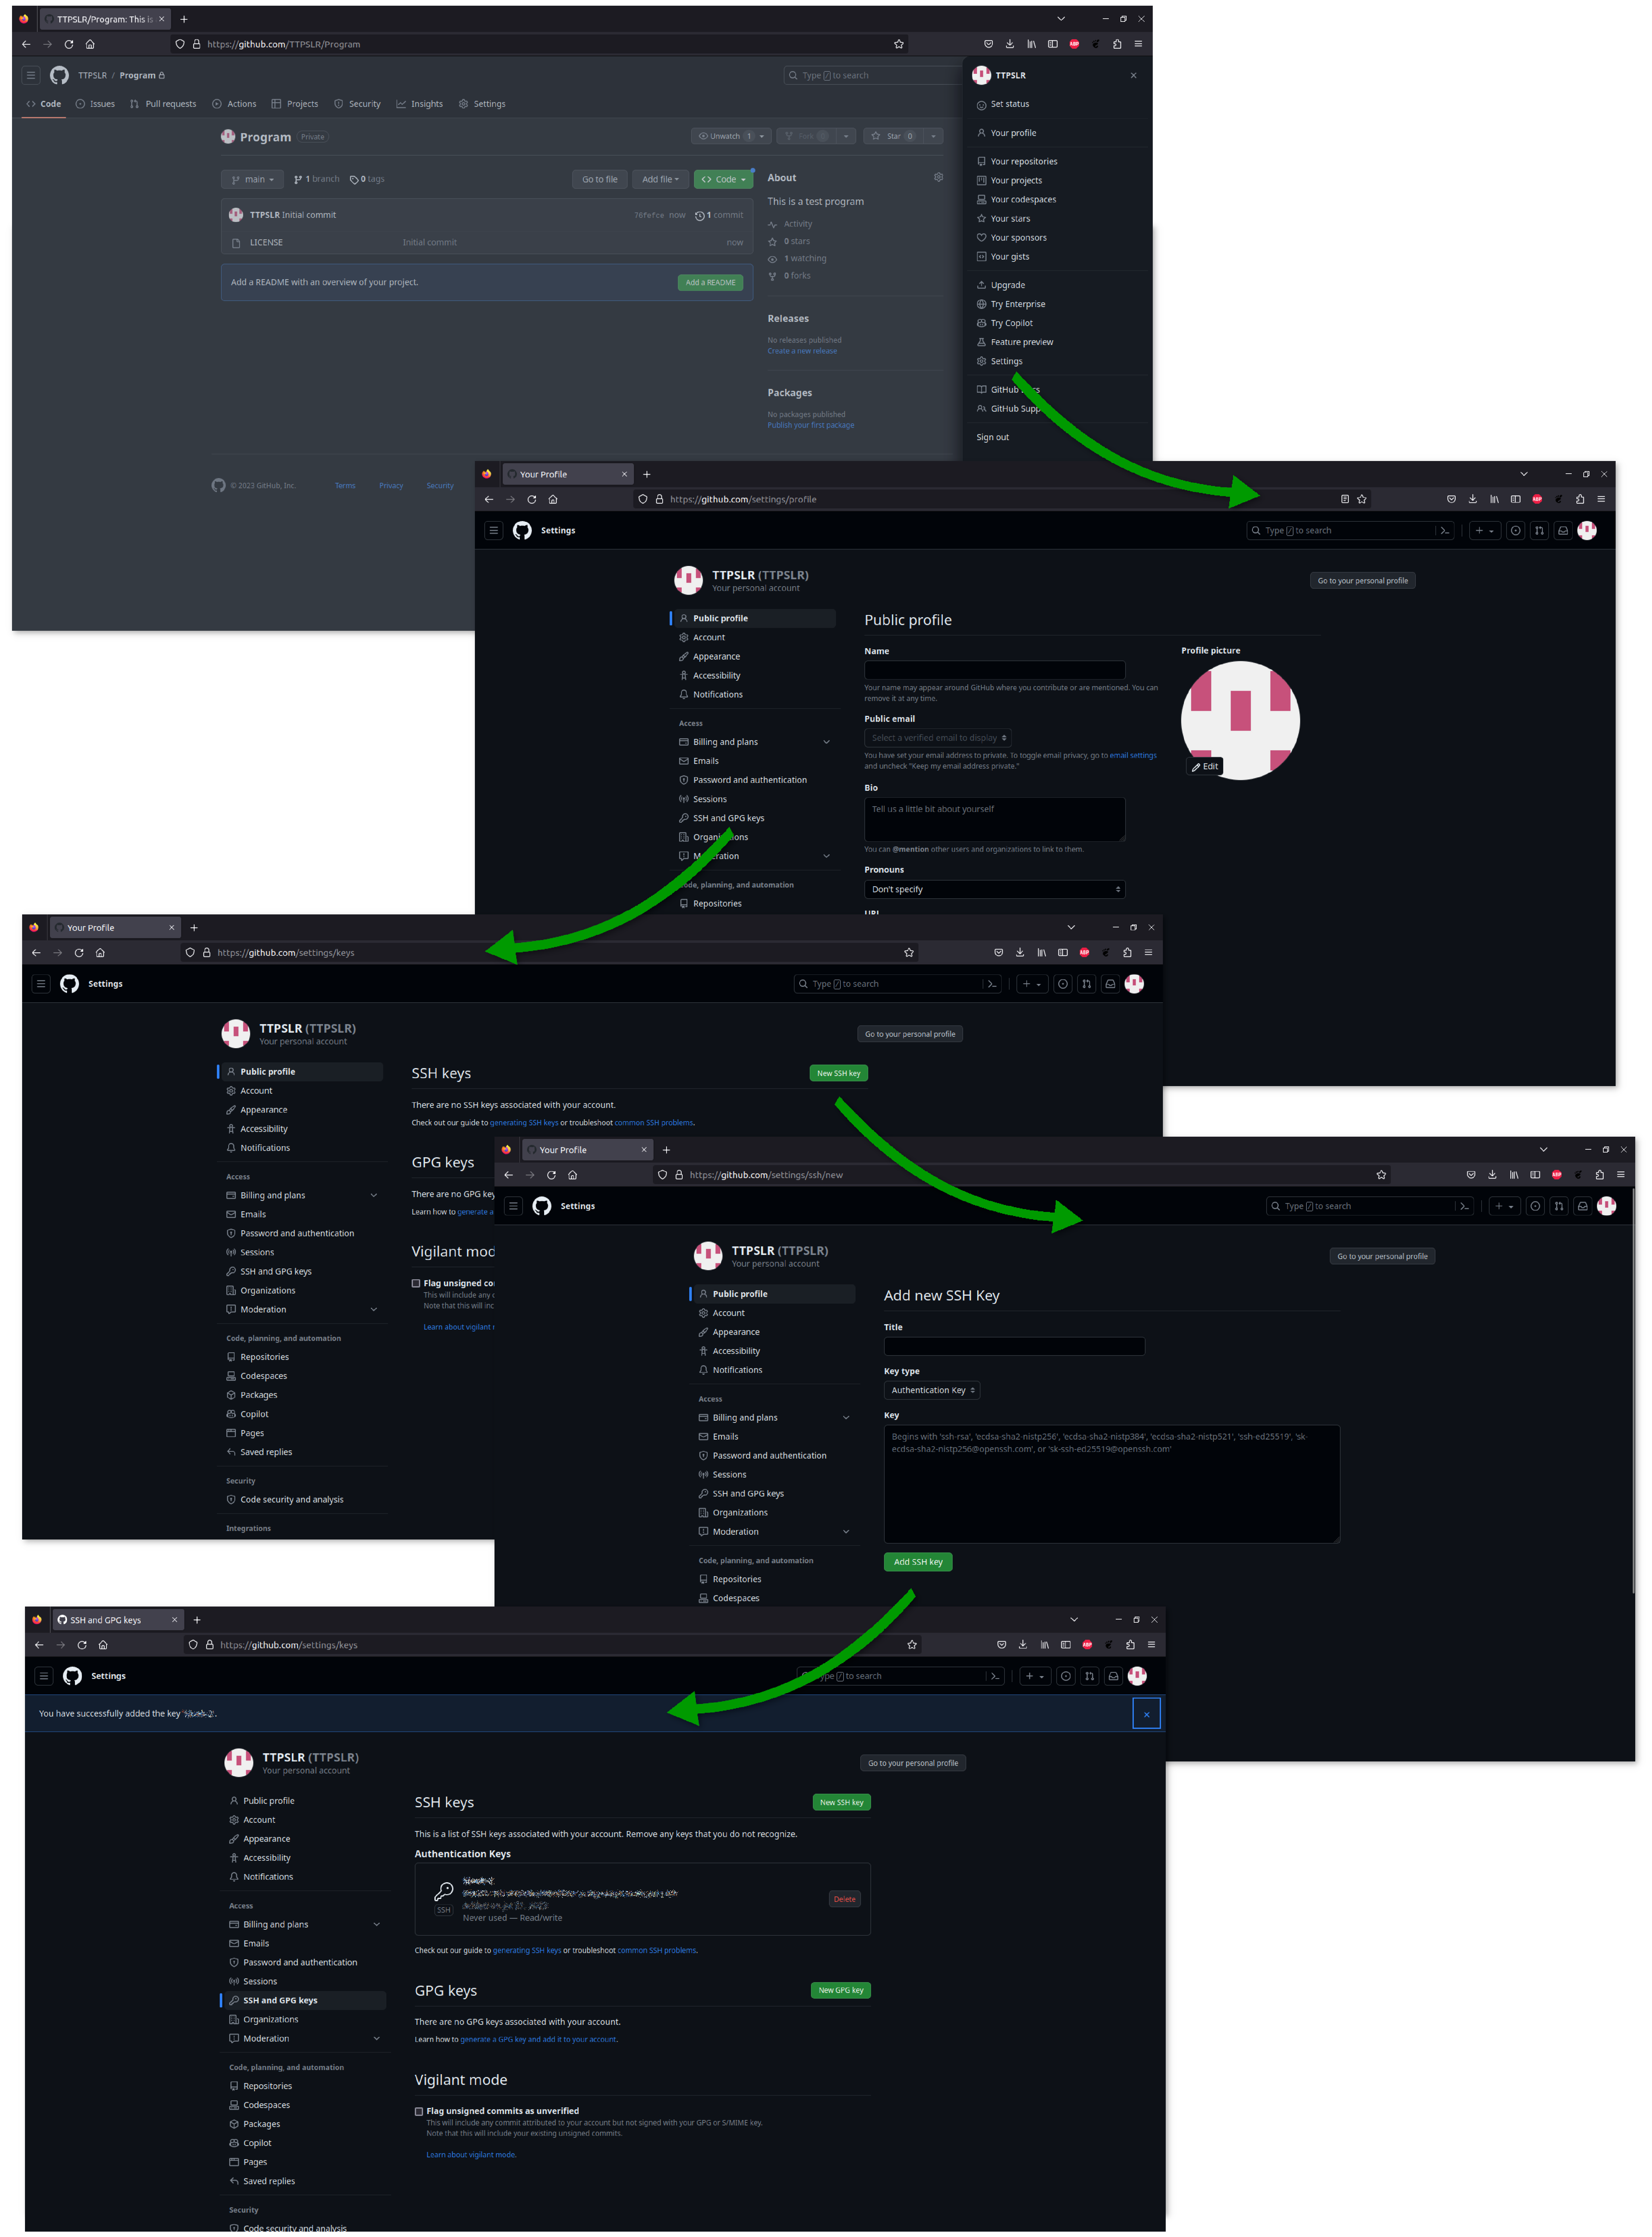
\includegraphics[width=1.0\textwidth,keepaspectratio=true,draft=\ddst]{img/hosts/github/keys.eps} 
\caption{Adding a SSH key on \github\label{kgithub}}
\end{figure}

\begin{figure}[!p]

\includegraphics[width=1.0\textwidth,keepaspectratio=true,draft=\ddst]{img/hosts/gitlab/keys.eps} 
\caption{Adding a SSH key on \gitlab\label{kgitlab}}
\end{figure}

\clearpage

\section{Branch protection}

If you are managing collaborative project, with several developers being able to push commits to the Git (and \github\ or \gitlab) repository branch(es), 
then you need to ensure that branch(es) of your project is (are) being protected against errors, ensuring that changes are handled by the project manager, or designated and selected developers. \\
To do that you need to enable, and adjust, branch(es) protection:
\begin{itemize}
\item \github\ (see figure~\ref{bgithub}):
\begin{itemize}
\item Click on "\texttt{Settings}"
\item Click on "\texttt{Branches}"
\item Click on "\texttt{Add branch protection rule}"
\item Choose branch name and adjust the protection level for this target branch of your project
\item Scroll down and click on "\texttt{Create}"
\end{itemize}
Note that on \github\ no branch protection is in place at the beginning to this step is really important. 
\item \gitlab:
\begin{itemize}
\item Default main branch protection for all your projects (see figure~\ref{mbgitlab}):
\begin{itemize}
\item Click on "\texttt{Settings}" $\Longrightarrow$ "\texttt{Repository}"
\item In front of "\texttt{Default branch}" click on "\texttt{Expand}"
\item Ensure that "\texttt{Fully protected}" 
\end{itemize}
\item Other branches protection (see figure~\ref{bpgitlab}):
\begin{itemize}
\item Click on "\texttt{Settings}" $\Longrightarrow$ "\texttt{Repository}"
\item In front of "\texttt{Protected branches}" click on "\texttt{Expand}"
\item Adjust the protection level for the target branch of your project
\end{itemize}
\end{itemize}
On \gitlab\ however branch protection should already be in place for the main branch.
\end{itemize}

\begin{figure}[!p]
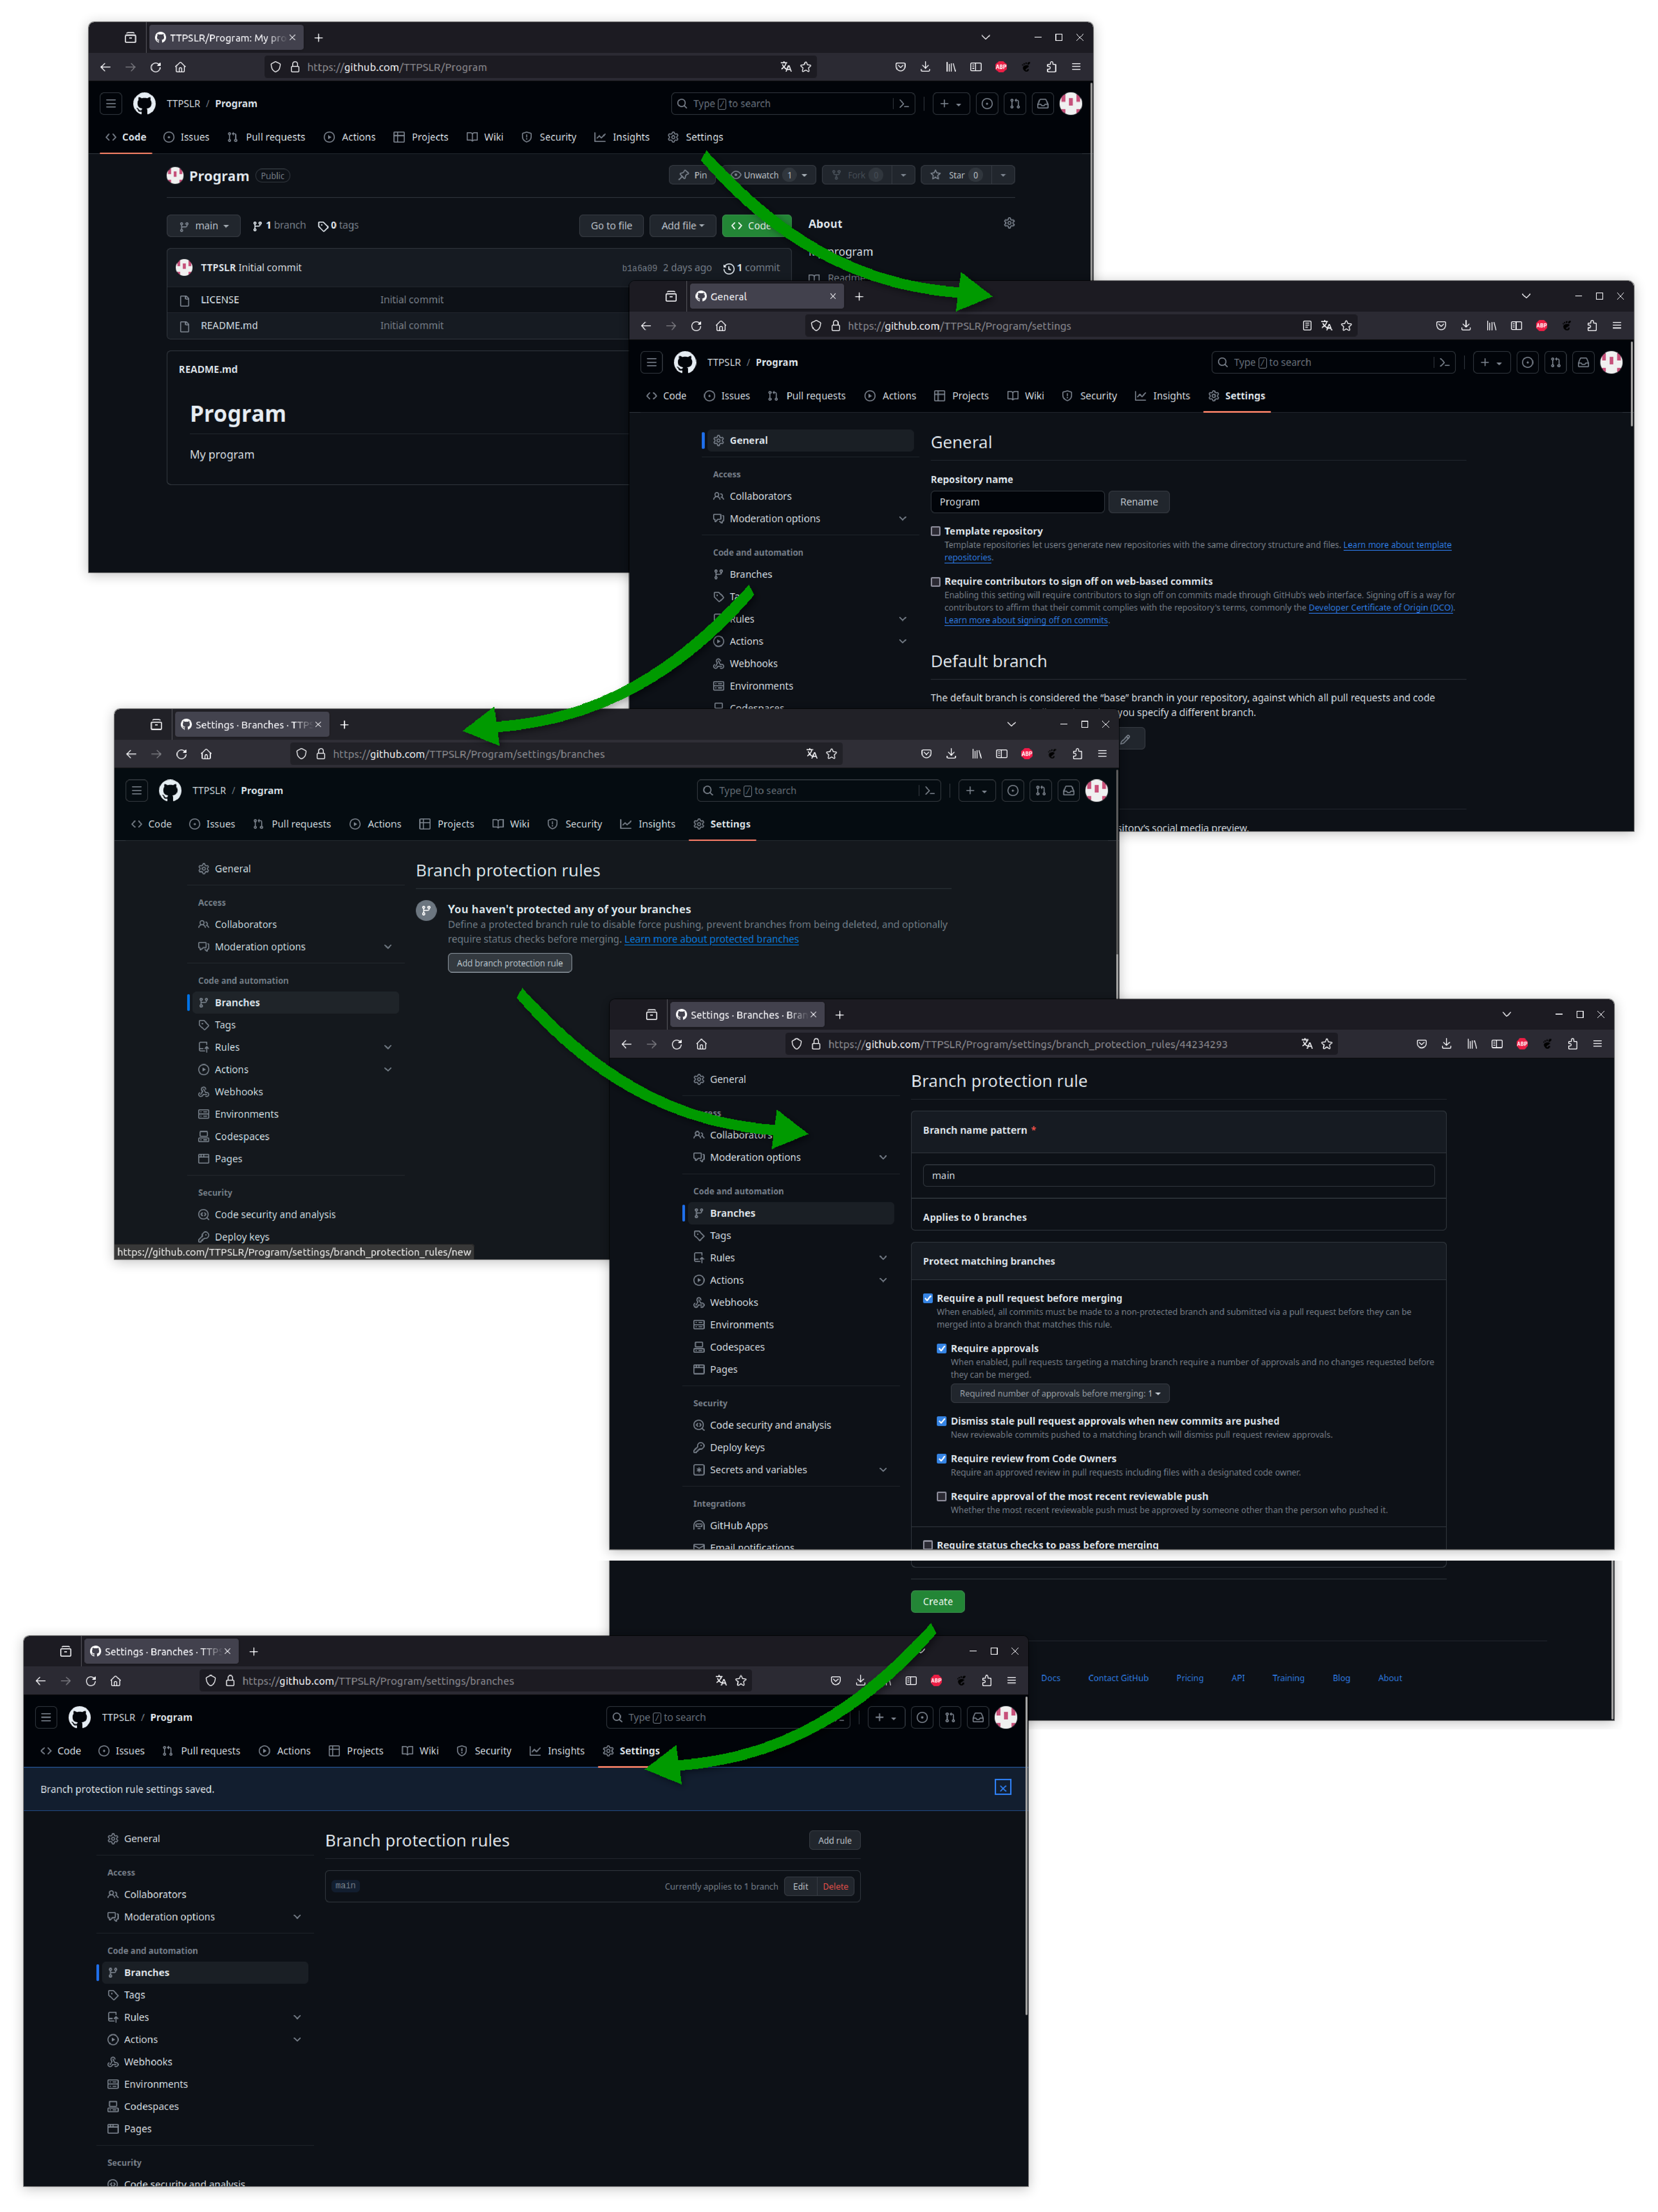
\includegraphics[width=1.0\textwidth,keepaspectratio=true,draft=\ddst]{img/hosts/github/branch.eps} 
\caption{Project branch projection on \github\label{bgithub}}
\end{figure}

\begin{figure}[!p]
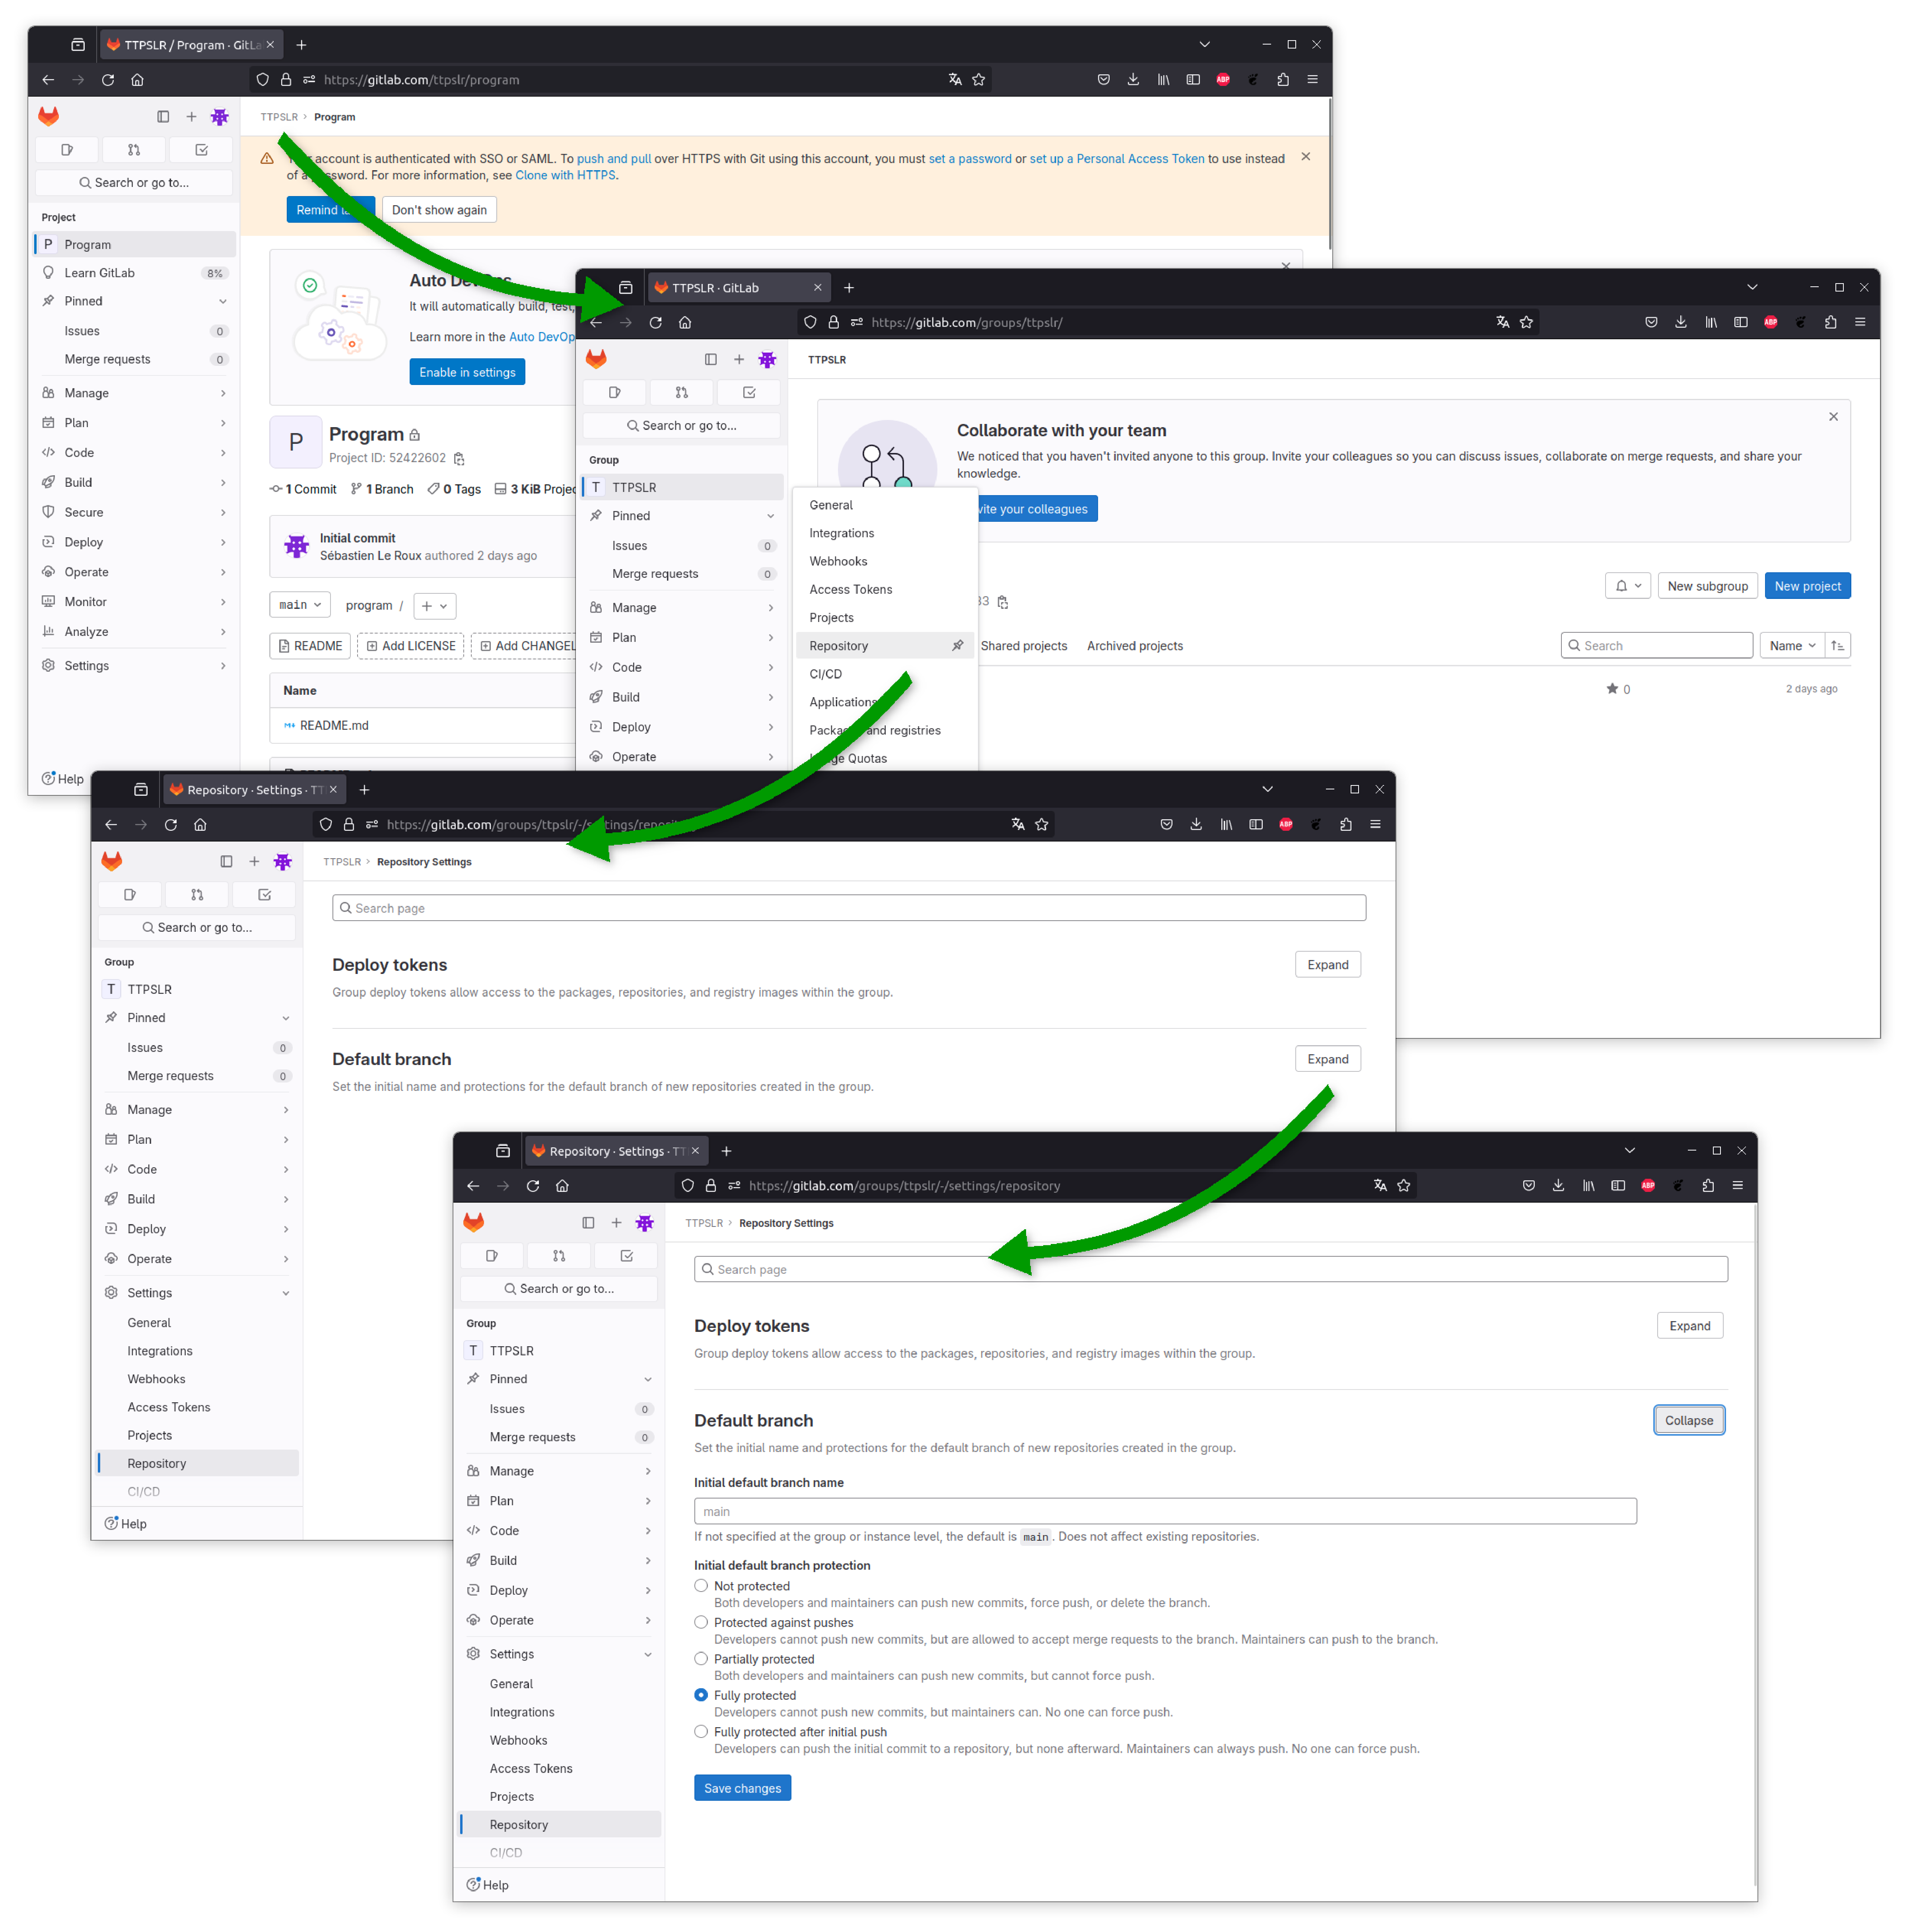
\includegraphics[width=1.0\textwidth,keepaspectratio=true,draft=\ddst]{img/hosts/gitlab/dbranch.eps} 
\caption{Default main branch projection on \gitlab\label{mbgitlab}}
\end{figure}

\begin{figure}[!p]
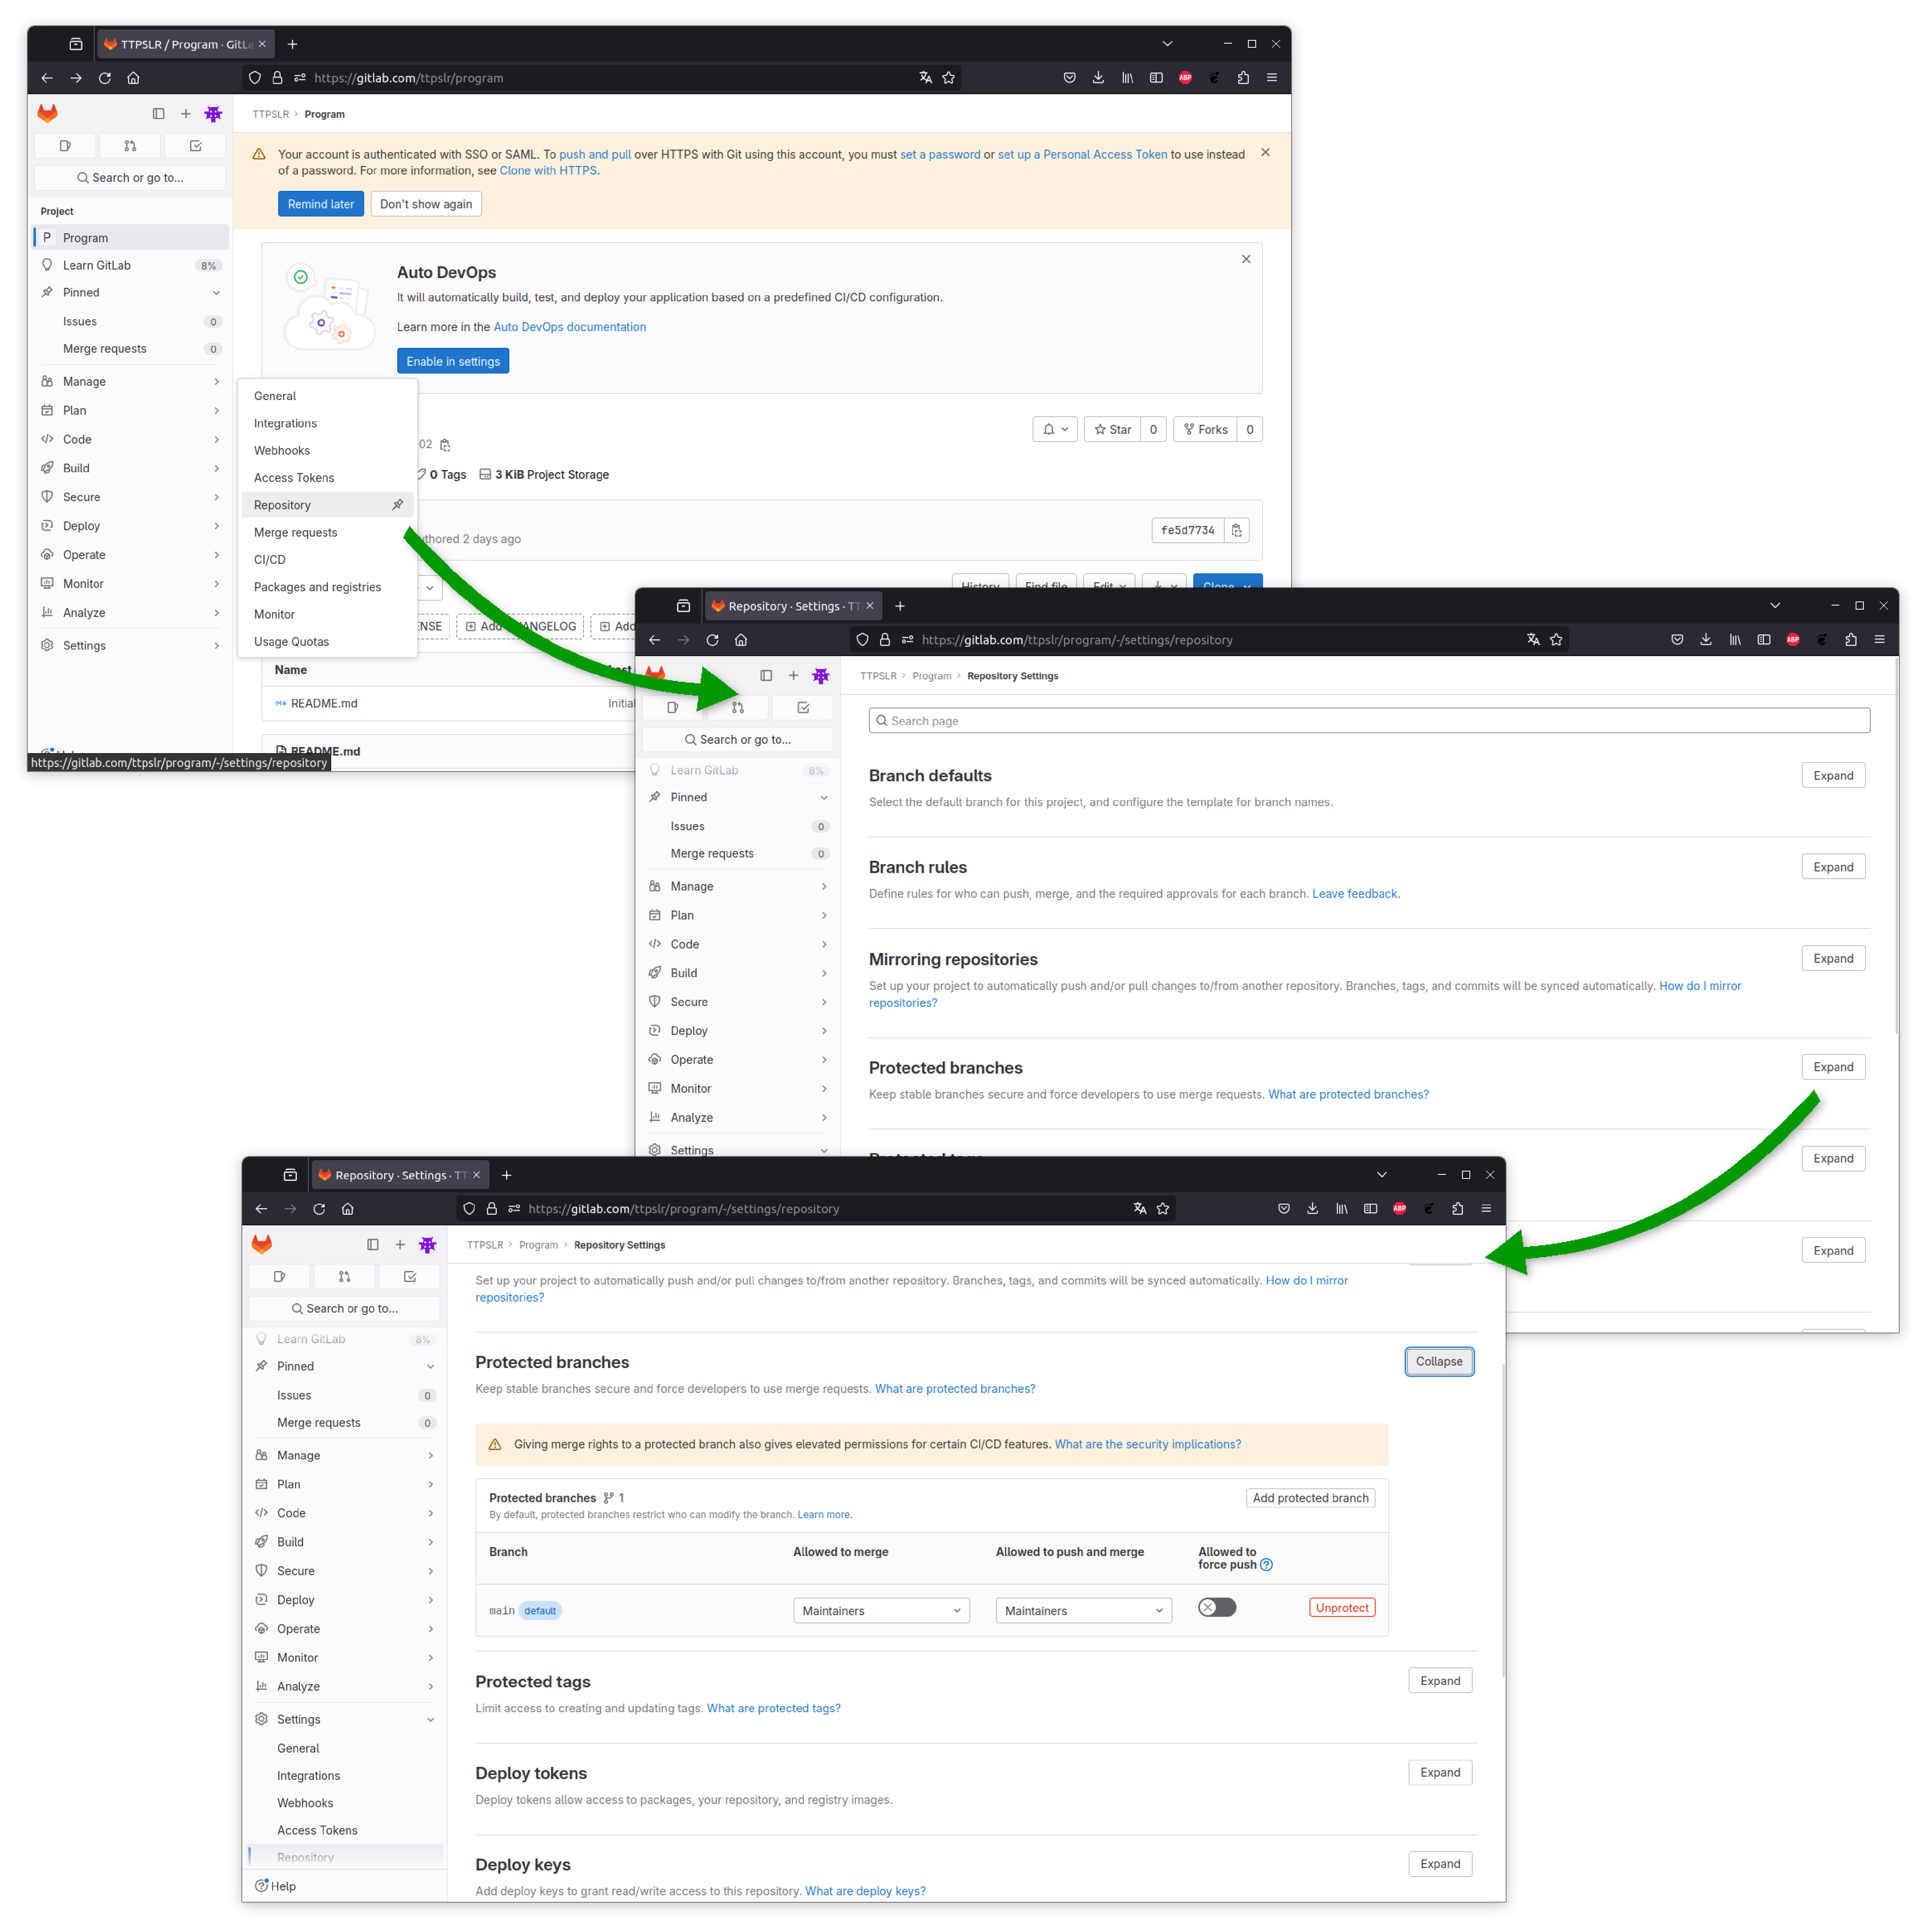
\includegraphics[width=1.0\textwidth,keepaspectratio=true,draft=\ddst]{img/hosts/gitlab/branch.eps} 
\caption{Project branch projection on \gitlab\label{bpgitlab}}
\end{figure}

\clearpage

\section{Releases and Tags}

\subsection{Tags}
\label{gtags}

On \github\ and \gitlab\ tags are images of the Git repository pointing towards archives that never change, 
like snapshots of the repository. \\
In both \github\ and \gitlab\ you can create tags whenever you think it is appropriate, 
however tags being required to produce a release, and a specific tag being associated with a specific release 
I will only focus thereafter in creating tag whenever creating release is required. 

\subsection{Releases}

On \github\ and \gitlab\ releases are deployable software versions made available for users to download. 
Releases are based on tags targeting specific points in the history of the repository. \\
To create a release: 
\begin{itemize}
\item On \github\ (see figure~\ref{rgithub}):
\begin{itemize}
\item Click on "\texttt{Create a new release}"
\item Click on "\bftt{Choose a tag}" to open the corresponding combo box:
\begin{itemize}
\item Input the new tag name, ex: "\texttt{1.0.0}" 
\item If the tag is new it is immediately proposed to create this tag
\item Click on "\bftt{Create new tag:} \bftt{1.0.0} \texttt{on publish}" \\
(or any other tag name of your choice)
\end{itemize}
\item Fill the description of the release, including release notes
\item Scroll down and click on "\texttt{Publish release}"
\end{itemize}
On \github\ releases packages have the form: "\rtt{tag}\bftt{.tar.gz}" \\
Extracting the archive on your hard drive will create a folder named: "\dgtt{repository-}\rtt{tag}"
\item On \gitlab\ (see figure~\ref{rgitlab}):
\begin{itemize}
\item On the left side menu, click on "\texttt{Deploy}" $\Longrightarrow$ "\texttt{Releases}"
\item Then click on "\texttt{Create a new release}"
\item Click on "\bftt{Tag name} \texttt{(required)}" to open the corresponding combo box:
\begin{itemize}
\item Input the new tag name, ex: "\texttt{1.0.0}" 
\item If the tag is new it is immediately proposed to create this tag
\item Click on "\texttt{Create tag} \bftt{1.0.0}" (or any other tag name of your choice)
\item Click on "\texttt{Save}"
\end{itemize}
\item Fill the description of the release, including release notes
\item Scroll down and click on "\texttt{Create release}"
\end{itemize}
On \gitlab\ releases packages have the form: "\dgtt{project}-\rtt{tag}\bftt{.tar.gz}" \\
Extracting the archive on your hard drive will create a folder named: "\dgtt{project-}\rtt{tag}"
\end{itemize}

\begin{figure}[!p]
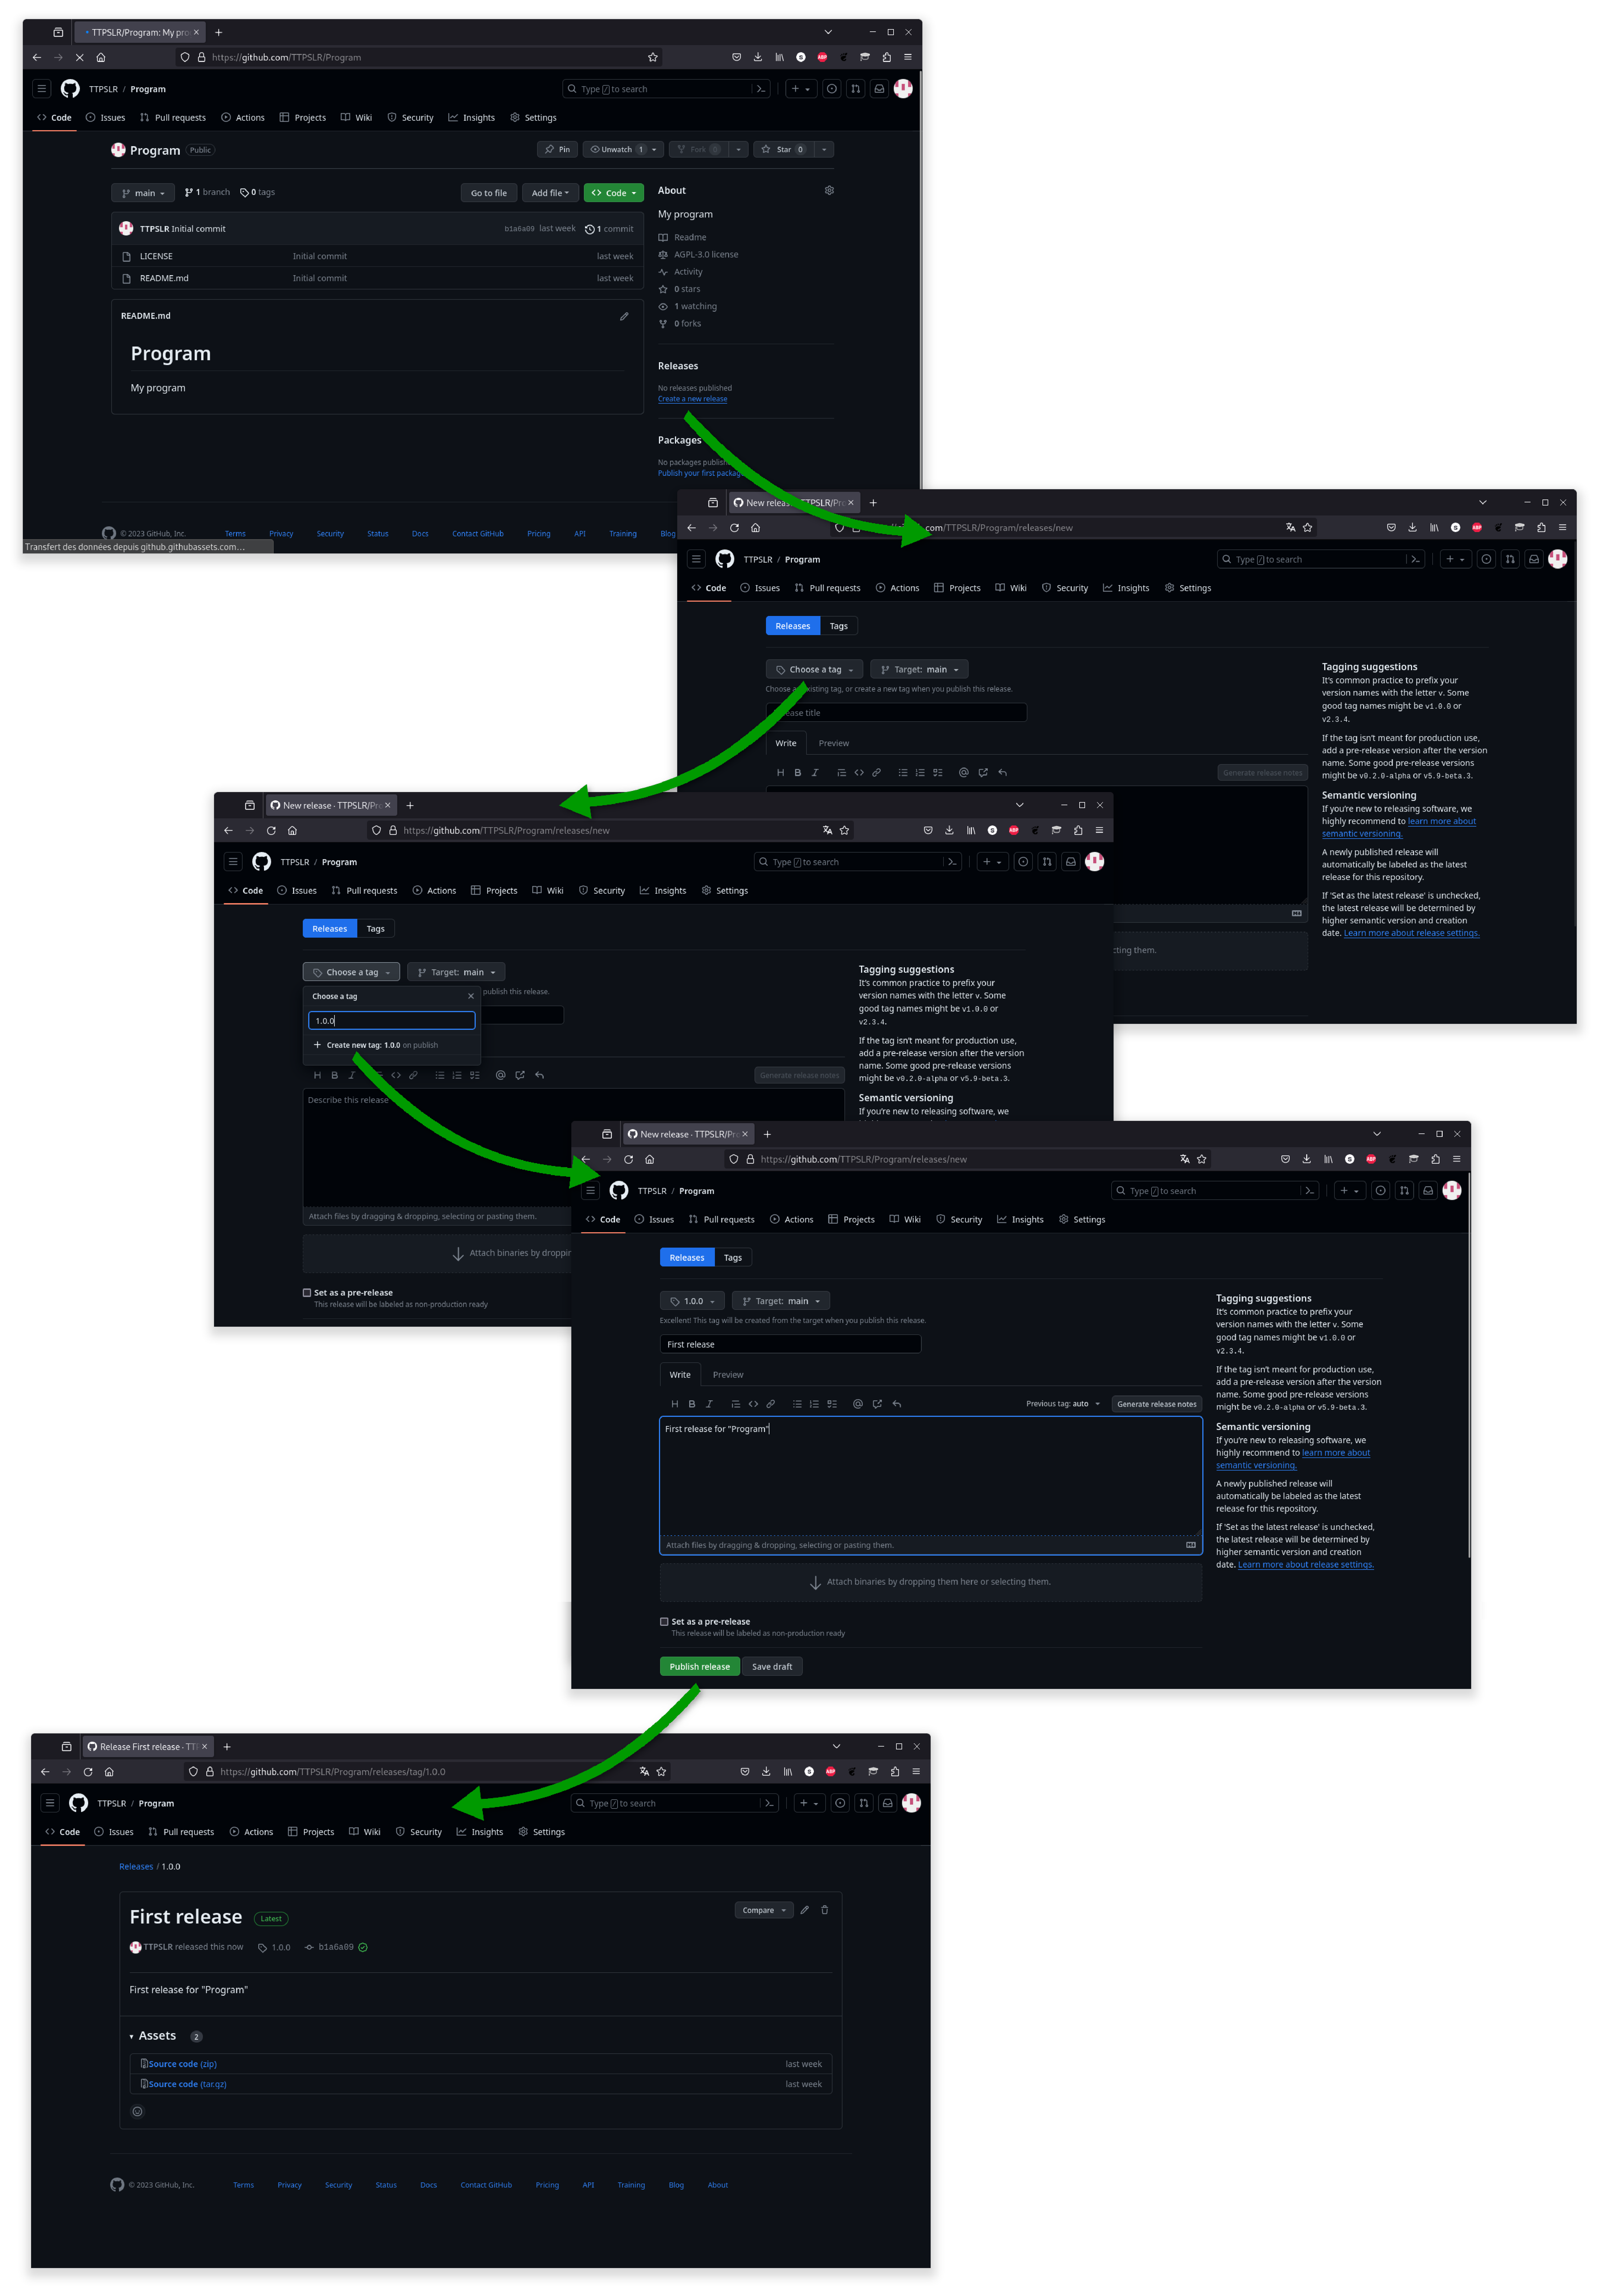
\includegraphics[width=1.0\textwidth,keepaspectratio=true,draft=\ddst]{img/hosts/github/release.eps} 
\caption{Creating a release on \github\label{rgithub}}
\end{figure}

\begin{figure}[!p]

\includegraphics[width=1.0\textwidth,keepaspectratio=true,draft=\ddst]{img/hosts/gitlab/release.eps} 
\caption{Creating a release on \gitlab\label{rgitlab}}
\end{figure}

\clearpage

\section{Using Git to manage your GitHub / GitLab project}
\label{onlinegit}

\subsection{Setting up work on you local computer} 

To start working on a remote repository using Git you can:
\begin{itemize}
\item {\bf{Clone}} the distant repository:
\begin{itemize}
\item \github:
{\footnotesize{
\begin{scriptii}
\fprompt{~/program} \bftt{git clone} git@github.com:\rtt{Author}/\btt{Program}
\end{scriptii}
}}
\item \gitlab:
{\footnotesize{
\begin{scriptii}
\fprompt{~/program} \bftt{git clone} git@gitlab.com:\rtt{Group}/\btt{Program}
\end{scriptii}
}}
\end{itemize}
\noindent Be careful \red{{\bf{NOT}}} to clone the distant repository using the "\texttt{https://git***}" instruction 
(both options being offered by \github\ and \gitlab), 
this would modify the access to the repository via the Git command line and require additional security considerations to setup 
developer access tokens, not considered in this manual. 
\item Alternatively set up manually the local folder to work remotely:
{\footnotesize{
\begin{scripti}
\fprompt{~} \bftt{mkdir} program
\fprompt{~} \bftt{cd} program
\fprompt{~/program} \bftt{git init}
\end{scripti}
}}
\begin{itemize}
\vspace{-0.5cm}
\item \github:
{\notsofoot{
\begin{scriptii}
\fprompt{~/program} \bftt{git remote} add origin git@github.com:\rtt{Author}/\btt{Program}
\end{scriptii}
}}
\\[-0.75cm]
\noindent Replace:
\begin{itemize}
\item \rtt{Name}\quad by the GitHub account that owns the repository.
\item \btt{Program}\quad by the name of the repository. \\
\end{itemize}
\item \gitlab:
{\notsofoot{
\begin{scriptii}
\fprompt{~/program} \bftt{git remote} add origin git@gitlab.com:\rtt{Group}/\btt{Program}
\end{scriptii}
}}
\\[-0.75cm]
\noindent Replace:
\begin{itemize}
\item \rtt{Group}\quad by the group Id for the GitLab account that owns the project.
\item \btt{Program}\quad by the name of the project. \\
\end{itemize}
\end{itemize}
This should be enough to get you started, providing that you check that the git user name and email are set properly (see [Sec.~\ref{gitconfig}]). \\[0.25cm]
Finally if needed setup the user information:
{\footnotesize{
\begin{scripti}
\fprompt{~} \bftt{git} \rtt{config} user.name "\abtt{Your Name}"
\fprompt{~} \bftt{git} \rtt{config} user.email \dctt{\email}
\end{scripti}
}}
\\[-0.75cm]
\noindent Replace:
\begin{itemize}
\item \rtt{Your Name}\quad by your user name. 
\item \btt{\email}\quad by your email. \\
\end{itemize}
Update the local folder with the content of the remote repository:
{\footnotesize{
\begin{scripti}
\fprompt{~/program} \bftt{git pull} origin \rtt{branch}
\end{scripti}
}}
\\[-0.75cm]
\noindent Replace:
\begin{itemize}
\item \rtt{branch}\quad by the branch of the project your are working on. 
\end{itemize} 
\end{itemize}
When this is done you can verify the link between your local folder and the on-line repository using:
\begin{script}
\fprompt{~/program} \bftt{git} remote -v
origin	git@github.com:\rtt{Author}/\btt{Program} (fetch)
origin	git@github.com:\rtt{Author}/\btt{Program} (push)
\end{script}
\\[-0.5cm]
\noindent Where:
\begin{itemize}
\item \rtt{Author}\quad is the GitHub account that owns the repository.
\item \btt{Program}\quad is the name of the repository. 
\end{itemize}

\subsection{Contributing to other project(s) and collaborative work}

If you want to work on project hosted on \github\ or \gitlab, and that you are not managing the project you intend to work on, then you need first to {\bf{fork}} this project. 
That means to create your own personnal copy of this project, independent of the original repository. \\
Afterwards to submit your modification(s) to the main repository you will need to create a dedicated branch and request to merge your branch to the main project. 
Modification(s) will be checked by a project manager, and if appropriate will be merged to the main branch of the repository. 
\newpage
\noindent To fork an exisiting project:
\begin{itemize}
\item On \github\ (see figure~\ref{fgithub}):
\begin{itemize}
\item Navigate to the \github\ project page of the repository you want to fork
\item Click on "\texttt{Fork}" to open the scrolling menu, and select "\texttt{Create a new fork}"
\item Follow the dialog to create a fork on the project in your own repository, you can select a specific branch if required, then when ready click on "\texttt{Create fork}"
\item It's done your own fork of the target project is now ready for you to work on in your own \github\ repository. 
\end{itemize}
\item On \gitlab\ (see figure~\ref{fgitlab}):
\begin{itemize}
\item Navigate to the \gitlab\ project page of the repository you want to fork
\item Click on "\texttt{Fork}"
\item Follow the dialog to create a fork on the project in your own repository, remember to specify the project URL. You can select a specific branch if required, then when ready click on "\texttt{Fork project}"
\item It's done your own fork of the target project is now ready for you to work on in your own \gitlab\ repository. 
\end{itemize}
\end{itemize}

\begin{figure}[!p]

\includegraphics[width=1.0\textwidth,keepaspectratio=true,draft=\ddst]{img/hosts/github/fork.eps} 
\caption{Creating a fork of a repository on \github\label{fgithub}}
\end{figure}
\begin{figure}[!p]

\includegraphics[width=1.0\textwidth,keepaspectratio=true,draft=\ddst]{img/hosts/gitlab/fork.eps} 
\caption{Creating a fork of a repository on \gitlab\label{fgitlab}}
\end{figure}

\newpage
\section{Project pages and documentation}

This section will illustrates how to use a \github\ / \gitlab\ repository and web pages to host a static web documentation for your project. 

\subsection{prerequisites}

It is required to install some tools to handle the publication of static webpages that will be used thereafter:
\begin{itemize}
\item Prepare the "\texttt{\textasciitilde/.bashrc}" file to install Ruby, insert the following lines:
\begin{scripti}
\fprompt{~} vi .bashrc
\comm{Install Ruby Gems to ~/gems}
\bad{export} \dctt{GEM\_HOME}\bad{=}\say{\$HOME/gems}
\bad{export} \dctt{PATH}\bad{=}\say{\$HOME/gems/bin:\$PATH}
\bad{export} \dctt{PATH}\bad{=}\say{\$HOME/.rbenv/bin:\$PATH}
\bftt{eval} \say{\$(rbenv init -)}
\bad{export} \dctt{PATH}\bad{=}\say{\$HOME/.rbenv/plugins/ruby-build/bin:\$PATH}
\end{scripti}
\item Install the Ruby dependencies (if needed)
\begin{itemize}
\item Fedora:
\vspace{-0.25cm}
{\footnotesize{
\begin{scriptii}
\textasciitilde]\$ \rtt{sudo} \bftt{dnf} install git-core gcc rust patch make bzip2 openssl-devel \textbackslash
                      libyaml-devel libffi-devel readline-devel zlib-devel \textbackslash
                      gdbm-devel ncurses-devel perl-FindBin perl-lib \textbackslash
                      perl-File-Compare
\end{scriptii}
}}
\item Debian:
\vspace{-0.25cm}
{\footnotesize{
\begin{scriptii}
\textasciitilde]\$ \rtt{sudo} \bftt{apt} install postgresql libpq-dev nodejs yarnpkg git zlib1g-dev \textbackslash
                      build-essential libssl-dev libreadline-dev libyaml-dev \textbackslash
                      libsqlite3-dev sqlite3 libxml2-dev libxslt1-dev \textbackslash
                      libcurl4-openssl-dev software-properties-common \textbackslash
                      libffi-dev
\end{scriptii}
}}
\end{itemize}
\item Install "\texttt{rbenv}":
{\footnotesize{
\begin{scripti}
\textasciitilde]\$ git clone https://github.com/rbenv/rbenv.git ~/.rbenv
\textasciitilde]\$ git clone https://github.com/rbenv/ruby-build.git ~/.rbenv/plugins/ruby-build
\textasciitilde]\$ \bftt{rbenv} \rtt{install} \dgtt{2.7.4}
\textasciitilde]\$ \bftt{rbenv} \rtt{global} \dgtt{2.7.4}
\textasciitilde]\$ \bftt{ruby} -v
\end{scripti}
}}
\\[-0.5cm]
\noindent \github\ pages are best compatible with version 2.7.x so do not install more recent release. \\
To list available stable versions:
{\footnotesize{
\begin{scripti}
\textasciitilde]\$ \bftt{rbenv} \rtt{install} \dctt{-l}
\end{scripti}
}}
\item Update "\texttt{rubygem}":
{\footnotesize{
\begin{scripti}
\textasciitilde]\$ \bftt{gem} \rtt{update} \dgtt{--system}
\end{scripti}
}}
\item Install \href{https://jekyllrb.com}{Jekyll} and the Ruby bundler:
\vspace{-0.25cm}
\begin{scripti}
\fprompt{~} \bftt{gem} \rtt{install} bundler jekyll
\end{scripti}
\end{itemize}
From this point forward the following steps are required to publish your documentation on \github\ or \gitlab\ pages:
\begin{enumerate}
\item Build the documentation of your project in \href{https://www.markdownguide.org/}{Markdown} and/or HTML language
\item Use Jekyll to convert your documentation in a static website
\item Create a repository on \github\ or \gitlab\ to host the documentation
\item Push your documentation to the web pages of the associated \github\ or \gitlab\ repository. 
\end{enumerate}

\subsection{Building the documentation in Markdown or HTML language}

It is up to you to decide how to do this, a good idea is to write your documentation in \LaTeX\ format, so that you can produce clean PDF documents. 
Then convert the \LaTeX\ files to HTML using \href{https://pandoc.org/}{pandoc}. \\
Also it allows to use your bibliography in Bib\TeX\ format and makes it easy to handle references on web pages. \\[0.25cm]
See the next section to know more about the data structure to prepare. \\[0.25cm]
Few things to take care of to use \LaTeX\ and \href{https://pandoc.org/}{pandoc} to prepare your documentation:
\begin{itemize}
\item To insert figures use PNG, or other graphic format, and not EPS as in standard \LaTeX\ documents. 
\item Be careful with the location of the images, ensure that the location, ideally in a separate and dedicated folder, 
matches the link in the HTML page. 
\item Internal references for objects not on the same HTML page will be lost when rendering the website. \\
This means that if your refer to a figure from the first chapter in the second chapter, likely on separate pages, 
you will have to correct the internal link to the proper web page. 
\item Pandoc conversion is not perfectly clean so few errors will likely require to be corrected afterwards, the best way 
to do that, is to understand the issue and to automate the correction process. \\
Among known errors to take care of:
\begin{itemize}
\item Check the table and figure captions
\item Some \LaTeX\ commands, in particular from peculiar custom packages, might not be understood by pandoc, and should be test proofed. \\[0.25cm]
For example the "\texttt{\textbackslash{Ctrl}}" command from the "\texttt{keystroke}" package (to render a drawing of the keyboard control key) 
cannot be processed by pandoc and should be replace by a command having the proper effect in HTML format, 
in this case "\texttt{\textbackslash{newcommand}\{\textbackslash{Ctrl}\}\{<kbd>Ctrl<\/kbd>\}}"
\end{itemize}
\item Finally to render \LaTeX\ math and equations in your HTML page insert the following code at the top of the HTML page:
\begin{itemize}
\item To render math using \href{https://www.mathjax.org/}{mathjax} use:
{\notsotiny{
\begin{scriptii}
\dbtt{<script} \abtt{src=}\red{"https://polyfill.io/v3/polyfill.min.js?features=es6"}\dbtt{></script>}
\dbtt{<script} \abtt{id=}\red{"MathJax-script" async src="https://cdn.jsdelivr.net/npm/mathjax@3.0.1/es5/tex-mml-chtml.js"}\dbtt{></script>}
\end{scriptii}
}}
\item To render math using \href{https://katex.org/}{katex} use:
{\notsotiny{
\begin{scriptii}
\dbtt{<script} \abtt{src=}\red{"https://cdnjs.cloudflare.com/ajax/libs/KaTeX/0.11.1/katex.min.js"}\dbtt{></script>}
\dbtt{<script>}document.addEventListener("DOMContentLoaded", function () {
   var mathElements = document.getElementsByClassName("math");
   var macros = [];
   for (var i = 0; i < mathElements.length; i++) {
      var texText = mathElements[i].firstChild;
      if (mathElements[i].tagName == "SPAN") {
       katex.render(texText.data, mathElements[i], {
        displayMode: mathElements[i].classList.contains({\textquotesingle}display{\textquotesingle}),
        throwOnError: false,
        macros: macros,
        fleqn: false
        });
      }}});
\dbtt{</script>}
\dbtt{<link} \abtt{rel=}\red{"stylesheet" href="https://cdnjs.cloudflare.com/ajax/libs/KaTeX/0.11.1/katex.min.css"} \dbtt{/>}
\dbtt{<!--}\abtt{[if lt IE 9]}\dbtt{>}
  \dbtt{<script} \abtt{src=}\red{"//cdnjs.cloudflare.com/ajax/libs/html5shiv/3.7.3/html5shiv-printshiv.min.js"}\dbtt{></script>}
\dbtt{<!}\abtt{[endif]}\dbtt{-->}
\end{scriptii}
}}
\end{itemize}
\end{itemize}
\vspace{-0.25cm}
Overall this method requires some additional work to properly convert the documents to a clean simple combination of Markdown and HTML structure, 
but once this work is automated you will only write your documentation using \LaTeX\ and then, in a single command, 
convert it and publish it to \github\ or \gitlab\ pages. 

\subsection{Using Jekyll to build a static website}

\href{https://jekyllrb.com}{Jekyll} is a simple static site generator. \\
Think of it like a file-based CMS, without all the complexity. Jekyll takes your content, renders Markdown and Liquid templates, 
and creates a complete, static website ready to be served by any web server. \\
Jekyll is the engine behind GitHub Pages, which you can use to host sites right from your GitHub repositories. \\[0.25cm]
Jekyll expects a document structure with Markdown files, but can also handles HTML files as includes files. 
In the following I will illustrate the document structure required by Jekyll to build a static web site: 
\begin{itemize}
\item For \LaTeX\ converted to HTML documentation
\item Using bibliography references in the \href{https://www.bibtex.org/}{Bib\TeX} format
\end{itemize}
Example repository to create the documentation: 
{\footnotesize{ 
\begin{script}
\fprompt{~/Program-doc} \bftt{ls}
\btt{\_bibliography}  \btt{chap-1}  \btt{intro}  \_config.yml  Gemfile  \btt{\_includes}  README.md
\end{script}
}}
\noindent With:
\begin{itemize}
\item Files:
\begin{itemize}
\item The home page of your documentation website: "\texttt{README.md}"
\item The list of Ruby extensions required to build your website: "\texttt{Gemfile}"
{\scriptsize{
\begin{scriptii}
\fprompt{~/Program-doc} \bftt{vi} Gemfile
source "\magenta{https://rubygems.org}"

\var{gem} {\textquotesingle}\magenta{jekyll-rtd-theme}{\textquotesingle}
\var{gem} {\textquotesingle}\magenta{github-pages}{\textquotesingle}, \magenta{group}: :\magenta{jekyll\_plugins}
\var{gem} {\textquotesingle}\magenta{jekyll-scholar}{\textquotesingle}, \magenta{group}: :\magenta{jekyll\_plugins}
group :\magenta{jekyll\_plugins} \bbtt{do}
  \var{gem} "\magenta{jekyll}", "\magenta{~> 3.9.0}"
  \var{gem} "\magenta{jekyll-feed}", "\magenta{~> 0.12}"
  \var{gem} "\magenta{jekyll-paginate}"
  \var{gem} "\magenta{jekyll-seo-tag}"
  \var{gem} "\magenta{jekyll-sitemap}"
  \var{gem} "\magenta{jekyll-archives}"
  \var{gem} "\magenta{jekyll-redirect-from}"
\bbtt{end}

\comm{Windows and JRuby does not include zoneinfo files,}
\comm{so bundle the tzinfo-data gem and associated library.}
platforms \magenta{:mingw}, \magenta{:x64\_mingw}, \magenta{:mswin}, \magenta{:jruby} \bbtt{do}
  \var{gem} "\magenta{tzinfo}", "\magenta{~> 1.2}"
  \var{gem} "\magenta{tzinfo-data}"
\bbtt{end}

\comm{ Performance-booster for watching directories on Windows}
\var{gem} "\magenta{wdm}", "\magenta{~> 0.1.1}", \magenta{:platforms} => [\magenta{:mingw}, \magenta{:x64\_mingw}, \magenta{:mswin}]
\end{scriptii}
}}
\item The Jekkyl configuration file to build the website: "\texttt{\_config.yml}"\\[-0.5cm] 
{\scriptsize{
\begin{scriptii}
\fprompt{~/Program-doc} \bftt{vi} \_config.yml
\var{title:} Program's documentation
\var{baseurl:} \magenta{"/Program-doc"}
\var{url:} \magenta{""}
\comm{GitHub or GtiLab repository:}
\var{repository:} TTPSLR/Program-doc
\var{lang:} en
\var{description:} This site presents the documentation for "Program"
\var{markdown:} kramdown
\var{highlighter:} rouge
\var{gist:}
  \var{noscript:} \magenta{false}
\var{kramdown:}
  \var{math\_engine:} mathjax
  \var{syntax\_highlighter:} rouge
\var{markdown\_extensions:}
  - \var{toc:}
    \var{permalink:} \magenta{"#"}
\comm{Define the depth of the menu}
    \var{baselevel:} 2
\var{banner:} \magenta{"/assets/img/banner.png"}
\var{favicon:} \magenta{"/assets/img/favicon.ico"}
\var{remote\_theme:} rundocs/jekyll-rtd-theme
\var{readme\_index:}
  \var{with\_frontmatter:} \magenta{true}

\var{plugins:}
  - jekyll-coffeescript
  - jekyll-default-layout
  - jekyll-gist
  - jekyll-github-metadata
  - jekyll-optional-front-matter
  - jekyll-paginate
  - jekyll-readme-index
  - jekyll-titles-from-headings
  - jekyll-relative-links
  - jekyll-scholar
  - jekyll-feed
  - jekyll-paginate
  - jekyll-seo-tag
  - jekyll-sitemap
  - jekyll-archives
  - jekyll-redirect-from
  - jekyll-remote-theme

\var{scholar:}
  \var{locale:} en
  \var{source:} ./\_bibliography
  \var{style:} \_bibliography/my-ieee.cls
  \var{bibliography:} references.bib
  \var{bibliography\_template:} \magenta{""}
  \var{replace\_strings:} \magenta{true}
  \var{join\_strings:}    \magenta{true}
  \var{use\_raw\_bibtex\_entry:} \magenta{false}
  \var{details\_dir:}    bibliography
  \var{details\_layout:} bibtex.html
  \var{details\_link:}   Details
\comm{Ensure that details are not printed twice}
  \var{query:} \magenta{"@*"}

\var{exclude:}
  - CNAME
  - Gemfile
  - Gemfile.lock
\end{scriptii}
}}
\end{itemize}
\item Directories:
\begin{itemize}
\item Each chapter or section in a separate directory, in this case "\btt{intro}" and "\btt{chap-1}":
\vspace{-0.25cm}
{\footnotesize{
\begin{scriptii}
\fprompt{~/program-doc} \bftt{ls} intro
README.md

\fprompt{~/program-doc} \lsr\ chap-1

chap-1:
README.md  \btt{section-1}  \btt{section-2}

chap-1/section-1:
README.md

chap-1/section-2:
README.md
\end{scriptii}
}}\\[-0.5cm]
\noindent Including sub-directories for chapter sections if required. \\
Note that each directory contains a single "\texttt{README.md}" file, dedicated to a single page of your site. \\[0.25cm]
\item Include files in the "\btt{\_includes}" directory:
{\footnotesize{
\begin{scriptii}
\fprompt{~/program-doc} \lsr\ \_includes
.:
\btt{intro}  \btt{chap-1}

./intro:
intro.html

./chap-1:
chap-1.html  \btt{section-1}  \btt{section-2}

./chap-1/section-1:
section-1.html

./chap-1/section-2:
section-2.html
\fprompt{~/program-doc}
\end{scriptii}
}} \\[-0.5cm]
\noindent including sub-directories for appendix chapters and sections if required. 
\newpage
\item The bibliography in the "\btt{\_bibliography}" directory:
{\footnotesize{
\begin{scriptii}
\fprompt{~/program-doc} \bftt{ls} \_bibliography
my-ieee.cls  references.bib
\end{scriptii}
}}
With:
\begin{itemize}
\item The "\texttt{*.ieee.cls}" file contains the bibliography style to apply
\item The "\texttt{*.bib}" file contains references in \href{https://www.bibtex.org/}{Bib\TeX} format \\
When you convert \LaTeX\ to HTML the keywords for the bibliography remain in the HTML document.
\end{itemize}
\end{itemize}
\end{itemize}
The "\texttt{README.md}" files, in Markdown format, follow the structure: 
{\footnotesize{
\begin{script}
\fprompt{~/program-doc} \bftt{vi} chap-1/README.md
\mdcom{This is a HTML comment in Markdown}
\mdcom{It will show up in the converted HTML document}

---
\mdcom{Position of this file in the website menu.}
\mdcom{To be compared will all other README.md file(s) at the same level,}
\mdcom{in this case all "~/program-doc/*/README.md" files}
sort: 2
\mdcom{Creation date:}
date: 2023-11-26
\mdcom{Math formula on this pages ?}
\mdcom{This is used to enable math javascript:}
maths: 1
---

\mdcom{# is the Markdown command for a heading}
\mdcom{Therefore the next line is the title of the chapter}
\magenta{# How to use "Program"}
\mdcom{Note if you do that you need to remove the heading line}
\mdcom{from the included HTML file bellow:}

\mdcom{Jekyll instruction to read an include file,}
\mdcom{and search for corresponding file(s) in the "\_include" folder}
\{\% include chap-1/chap-1.html \%\}

\mdcom{Jekyll instruction to process all sub-directories, if any:}
\{\% include list.liquid all=true \%\}

\mdcom{Jekyll instruction to add a bibliography section on this page:}
\{\% bibliography --cited \%\}
\mdcom{Then Jekyll search the "\_bibliography" folder to insert references}
\end{script}
}}
\clearpage
\noindent Jekyll will search for all "\texttt{README.md}" files in the directory tree, starting from the top directory. 
and build the website according to the "\texttt{sort}" instructions, in this example:
\begin{itemize}
\item Top level, homepage: "\texttt{README.md}"
\begin{itemize}
\item First level: \\
\begin{itemize}
\item In "\texttt{intro\textbackslash README.md}"  \,\,\ \quad$\Longrightarrow$\quad "\texttt{sort: }\rtt{1}"\\
\item In "\texttt{chap-\rtt{1}\textbackslash README.md}" \quad$\Longrightarrow$\quad "\texttt{sort: }\rtt{2}"\\
\item[$-$] Second level (chapter sections): \\
\begin{itemize}
\item In "\texttt{chap-1\textbackslash section-\rtt{1}\textbackslash README.md}" \quad$\Longrightarrow$\quad "\texttt{sort: }\rtt{1}"\\
\item In "\texttt{chap-1\textbackslash section-\rtt{2}\textbackslash README.md}" \quad$\Longrightarrow$\quad "\texttt{sort: }\rtt{2}"\\
\end{itemize}
\end{itemize}
\end{itemize}
\end{itemize}
Jekyll will create a HTML page for each "\texttt{README.md}" file found in the directory tree. \\
For your documentation to be easy to browse and read take time to organize it properly and split the pages accordingly. \\
The directories "\texttt{\_includes}" and "\texttt{\_bibliography}" are ignored by Jekyll when searching for "\texttt{README.md}" files, 
however their content is used to produce the website. \\[0.25cm]
To install the packages required by the "\texttt{Gemfile}" to build your site use:
\begin{script}
\fprompt{~/Program-doc} \bftt{bundle} \rtt{install}
\end{script}\\[-0.75cm]
\noindent Then to build the site use:
\begin{script}
\fprompt{~/Program-doc} \bftt{bundle} \rtt{exec} \dgtt{jekyll} build
\end{script}\\[-0.75cm]
\noindent You will see that this command creates a new directory name "\texttt{\_site}" that contains your website. 
\begin{script}
\fprompt{~/Program-doc} ls \_site

\end{script}\\[-0.75cm]
\noindent You can give a try to this website on your computer using: 
\begin{script}
\fprompt{~/Program-doc} \bftt{bundle} \rtt{exec} \dgtt{jekyll} serve
\end{script}\\[-0.75cm]
\noindent And simply follow the instructions.
\newpage

\subsection{Hosting the website on GitHub}

To use \github\ to host your documentation: 
\begin{itemize}
\item Create a dedicated repository, in the following example: "\texttt{TTPSLR/Program-doc}"
\item After properly configuring the connection to the remote repository, upload the contents of the "\texttt{\textasciitilde/Program-doc}" but the folder "\texttt{\_site}" to the main branch, separate branches allows to keep track of both the source material and the final content of the website:
\begin{scriptii}
\fprompt{~/Program-doc} \bftt{mv} \_site ../
\fprompt{~/Program-doc} \bftt{git} \rtt{checkout} \btt{-b} Main
\fprompt{~/Program-doc} \bftt{git} \rtt{add} .
\fprompt{~/Program-doc} \bftt{git} \rtt{commit} \btt{-m} "To build the doc"
\fprompt{~/Program-doc} \bftt{git} \rtt{push} \btt{origin} Main
\end{scriptii}
\item After properly configuring the connection to the remote repository, upload the contents of the "\texttt{\_site}" to the \github\ pages, the "\texttt{gh-pages}" branch:
\begin{scripti}
\fprompt{~/\_site} \bftt{git} \rtt{checkout} \btt{-b} gh-pages
\fprompt{~/\_site} \bftt{git} \rtt{add} .
\fprompt{~/\_site} \bftt{git} \rtt{commit} \btt{-m} "Documentation"
\fprompt{~/\_site} \bftt{git} \rtt{push} \btt{origin} gh-pages
\end{scripti}
\end{itemize}
After a short while the result is updated, and as is illustrated on figure~\ref{dgithub}, the website is alive. \\
Open the "\texttt{Pages}" tab in the "\texttt{Settings}" menu, to find out the web address of your site. \\
In this example: \href{https://ttpslr.github.io/Program-doc}{https://ttpslr.github.io/Program-doc} \\[0.25cm]
The \github\ pages address have the form:\quad https://\rtt{Author}.github.io/\btt{Program}

\begin{figure}[!p]
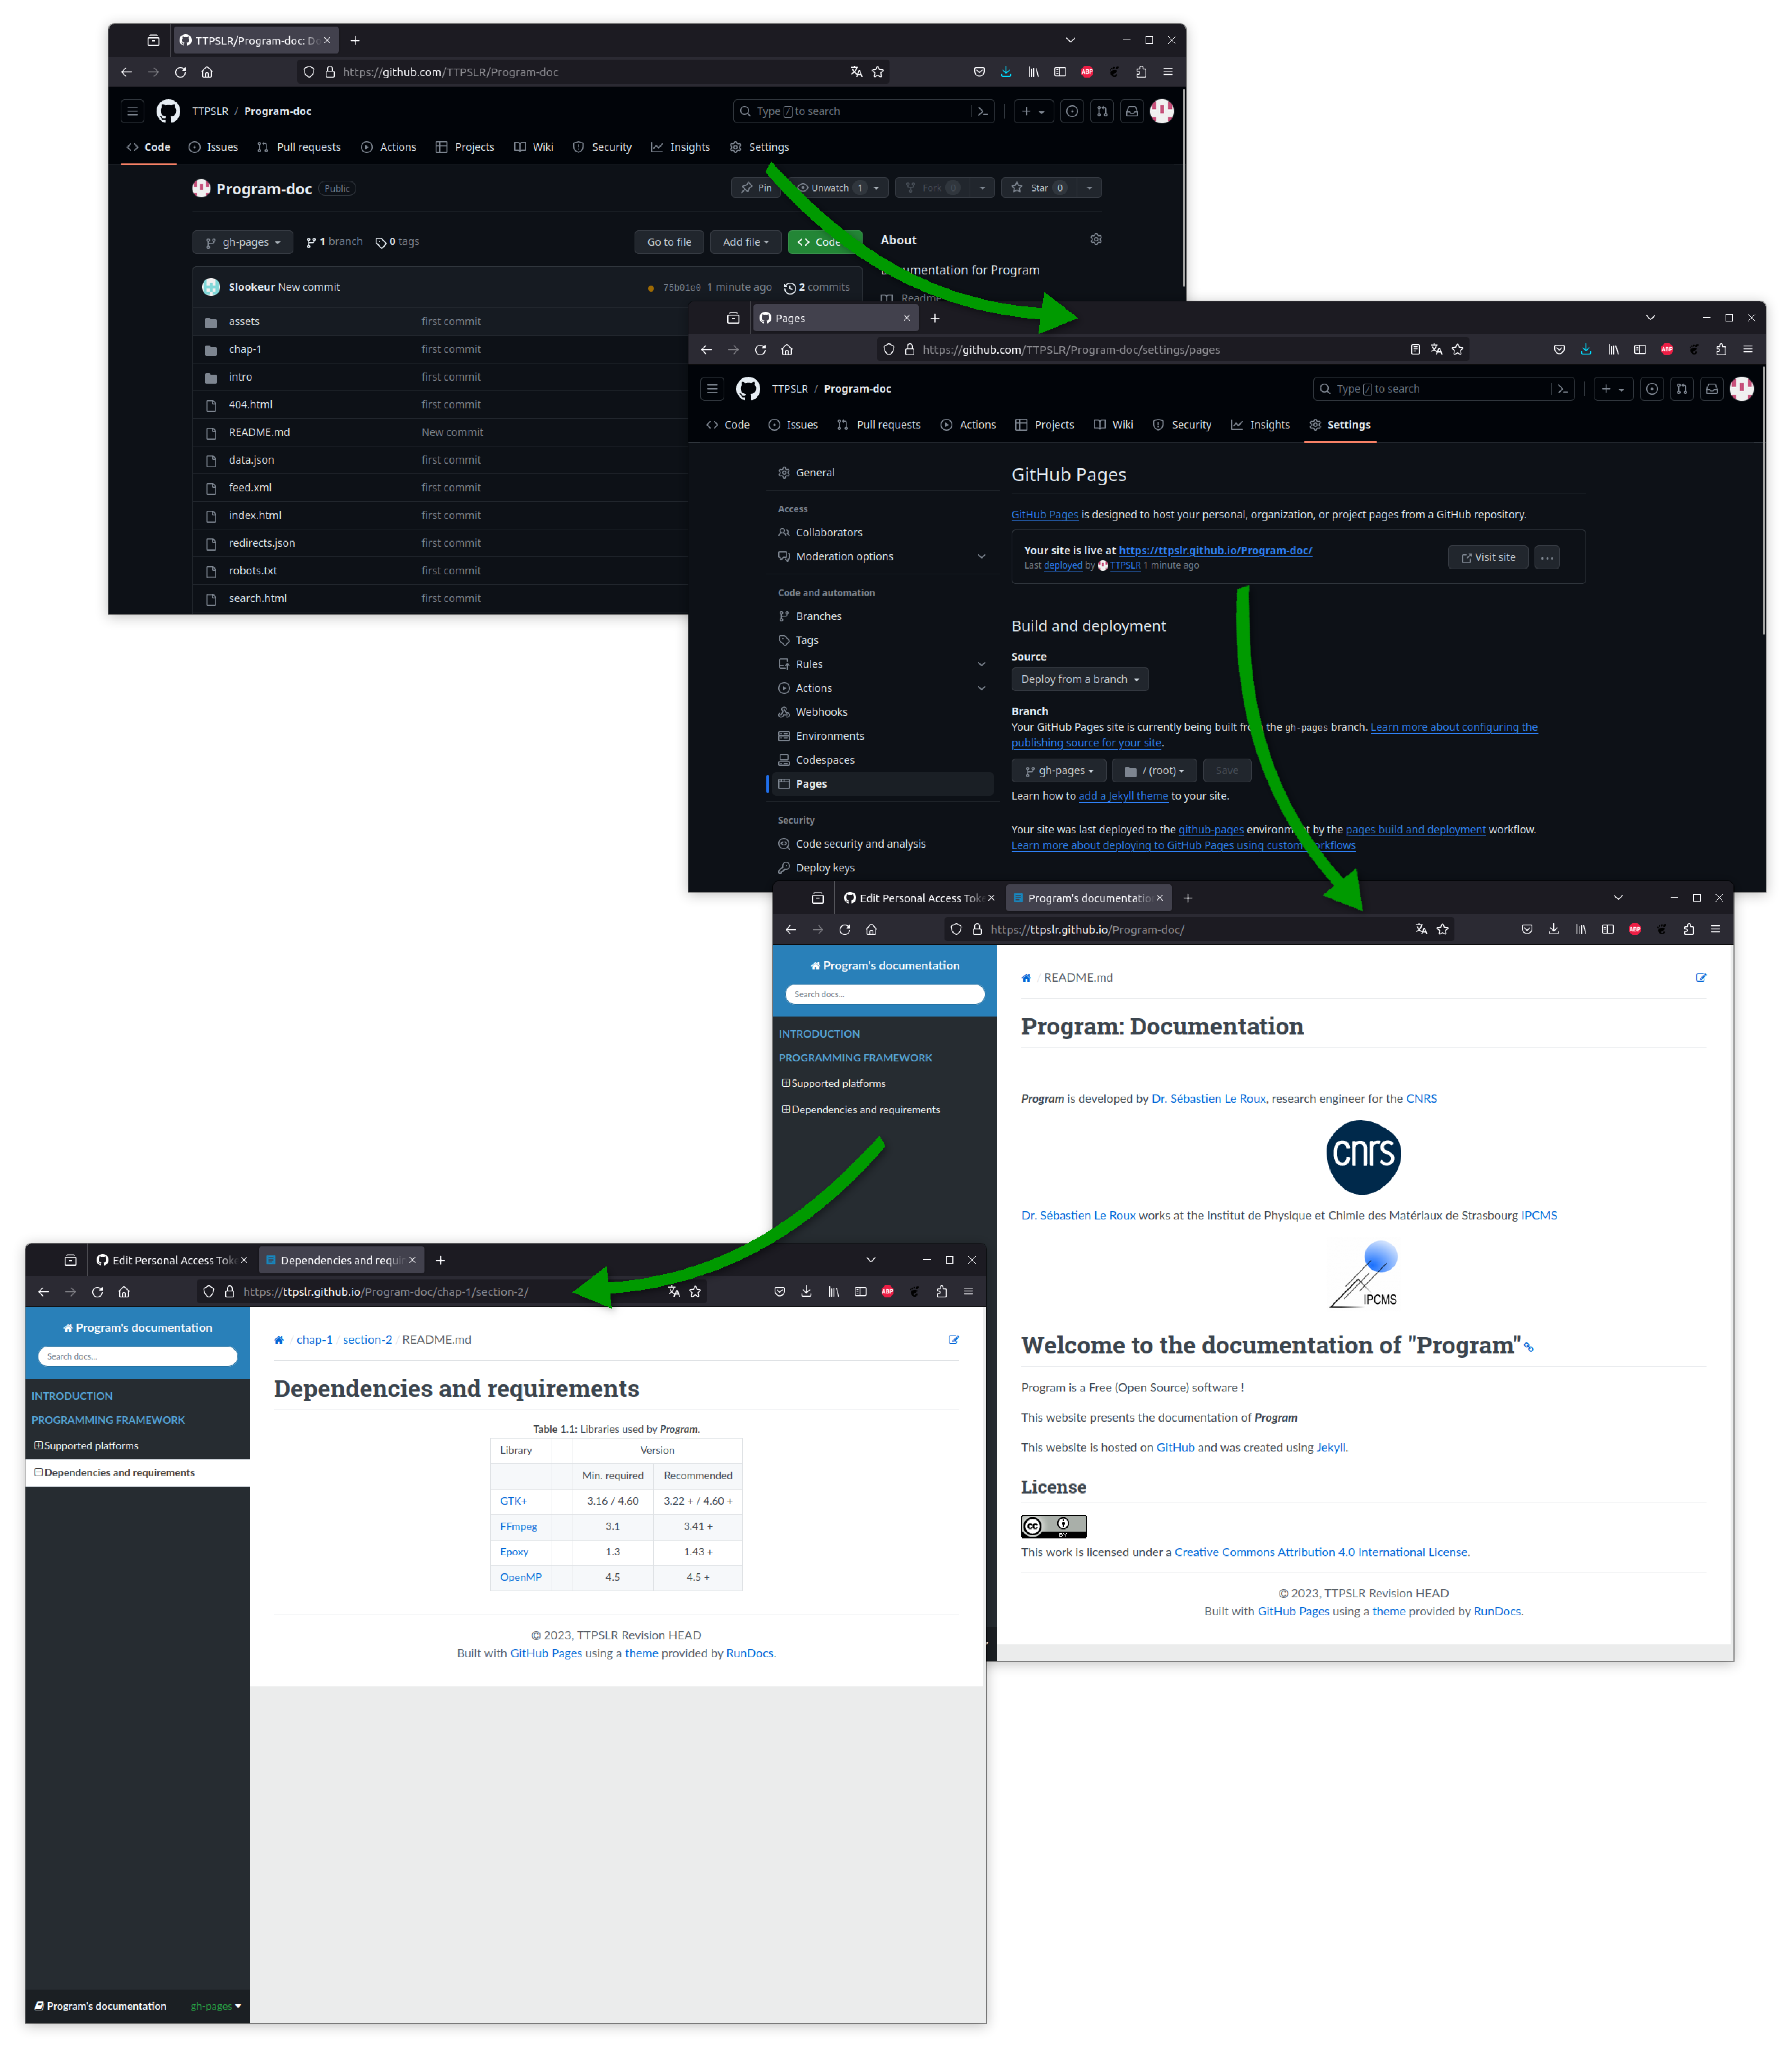
\includegraphics[width=1.0\textwidth,keepaspectratio=true,draft=\ddst]{img/hosts/github/doc.eps} 
\caption{Hosting the documentation on \github\label{dgithub}}
\end{figure}

